\documentclass[a4paper, 12pt, twoside]{article}
\usepackage[T2A,T1]{fontenc}
\usepackage[utf8]{inputenc}
\usepackage[english, russian]{babel}
\usepackage{graphicx}
\usepackage[hcentering, bindingoffset = 10mm, right = 15 mm, left = 15 mm, top=20mm, bottom = 20 mm]{geometry}
\usepackage{multirow}
\usepackage{ctable}
\usepackage{lipsum}
\usepackage{amsmath, amstext}
\usepackage{siunitx}
\usepackage{subcaption}
\usepackage{wrapfig}
\usepackage{adjustbox}
\usepackage{enumerate, indentfirst, float}
\usepackage{capt-of, svg}
\usepackage{cmap} % Улучшенный поиск русских слов в полученном pdf-файле

\usepackage{pscyr} % Нормальные шрифты
\usepackage[normalem]{ulem} % для подчёркиваний uline
\ULdepth = 0.16em
%% Перенос знаков в формулах (по Львовскому)
\newcommand*{\hm}[1]{#1\nobreak\discretionary{}
	{\hbox{$\mathsurround=0pt #1$}}{}}

\usepackage{fancyhdr} %Колонтикулы
\pagestyle{fancy}
\lhead{
\includegraphics[width = 10 mm]{logo.jpg} Применения операционных усилителей.}
\rhead{\textit{\today}}

\newenvironment{bottompar}{\par\vspace*{\fill}}{\clearpage}
 
\begin{document}
\begin{titlepage}

\newcommand{\HRule}{\rule{\linewidth}{0.7mm}} % Defines a new command for the horizontal lines, change thickness here

\center % Center everything on the page
 
%----------------------------------------------------------------------------------------
%	HEADING SECTIONS
%----------------------------------------------------------------------------------------

\textsc{\LARGE Московский Физико-Технический Институт}\\[1,5cm] % Name of your university/college

\textsc{\large Лабораторная работа по радиотехническим сигналам и цепям}\\[0.5cm] % Minor heading such as course title

%----------------------------------------------------------------------------------------
%	TITLE SECTION
%----------------------------------------------------------------------------------------

\HRule
\\[0.4cm]
{ \huge \bfseries Применение операционных усилителей.}
\\[0.4cm] % Title of your document
\HRule
\\[1.5cm]


 
%----------------------------------------------------------------------------------------
%	AUTHOR SECTION
%----------------------------------------------------------------------------------------


	\begin{center} \large
		\textbf{Автор:}\\
		Глеб Уваркин \\
		615 группа
	\end{center}

~


\begin{bottompar}
	\begin{center}
		
\includegraphics[width = 80 mm]{logo.jpg}
	\end{center}
	{\large \today}

\end{bottompar}
\vfill % Fill the rest of the page with whitespace

\end{titlepage}

\section*{Задание №1.Измерение коэффициента усиления ОУ.}

\begin{figure}[H]
	\centering
	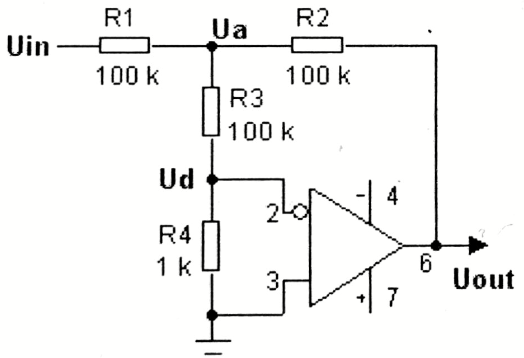
\includegraphics[width =  0.3\linewidth]{kus}
	\caption{Схема измерения коэффициента усиления.}
	\label{kus}

\end{figure}


Соберём схему, показанную на рис. \ref{kus}. Сопротивления резисторов возьмём: $R_1=R_2=R_3=200$ кОм, $R_4 = 2$ кОм, $R_3/R_4 = 100$.
\vspace{\baselineskip}

Подадим на вход колебание с амплитудой $U_{in} = 2.5$ В и частотой $f = 15$ Гц. Измерим величину напряжений $U_a$ и $U_{out}$: $U_a = 4.4 $ мВ, $U_{out} = 2.46$ В. 

\vspace{\baselineskip}

Рассчитаем коэффициент усиления операционного усилителя по формуле $A_0 = (1 \hm{+}R_3/R_4)\cdot (U_{out}/U_a)$:
$$A_0 = (1 + 100)\dfrac{2.46}{4.4\cdot 10^{-3}} = 56468  \simeq 6 \cdot 10^4$$.
\newpage
\section*{Задание №2. Амплитудно-частотная характеристика ОУ.}

Для схемы на рис. \ref{kus} снимем зависимость коэффициента усиления от частоты (АЧХ), используя формулу: $$A(f) = \dfrac{U_{out}}{U_d} = \dfrac{U_{out}}{U_a}\cdot \dfrac{U_a}{U_d} = \left(1+\dfrac{R_3}{R_4}\right )\cdot \dfrac{U_{out}}{U_a}.$$
Занесём полученные данные в таблицу \ref{kus}.

\begin{table}[H]
	\centering
	\caption{Зависимость коэффициента усиления от частоты.}
	\label{kus}
	\begin{tabular}{c|c|c|c|c|c|c|c|c|c|c}
		\toprule
		$f,$ Гц      & 50    & 100   & 200   & 500  & 1000 & 2000 & 5000 & 10000 & 20000 & 50000 \\ 
		$U_{out},$ В & 2.48  & 2.48  & 2.48  & 2.48 & 2.47 & 2.43 & 2.21 & 1.73  & 1.06  & 0.76  \\ 
		$U_a,$ мВ    & 5.55  & 8.67  & 16    & 39   & 77   & 152  & 343  & 543   & 131   & 119   \\ 
		$A$          & 45000 & 29000 & 16000 & 6000 & 3000 & 1600 & 651  & 324   & 82    & 65    \\ \midrule
		$lgf$        & 1.7   & 2     & 2.3   & 2.7  & 3    & 3.3  & 3.7  & 4     & 4.3   & 4.7   \\ 
		$20lgA,$ дБ      & 93    & 89    & 84    & 76   & 69   & 64   & 56   & 50    & 38    & 36    \\ \bottomrule
	\end{tabular}
\end{table}

Построим снятую зависимость в двойном логарифмическом масштабе, откладывая частоту в герцах, а коэффициент усиления в децибелах.

\begin{figure}[H]
	\centering
	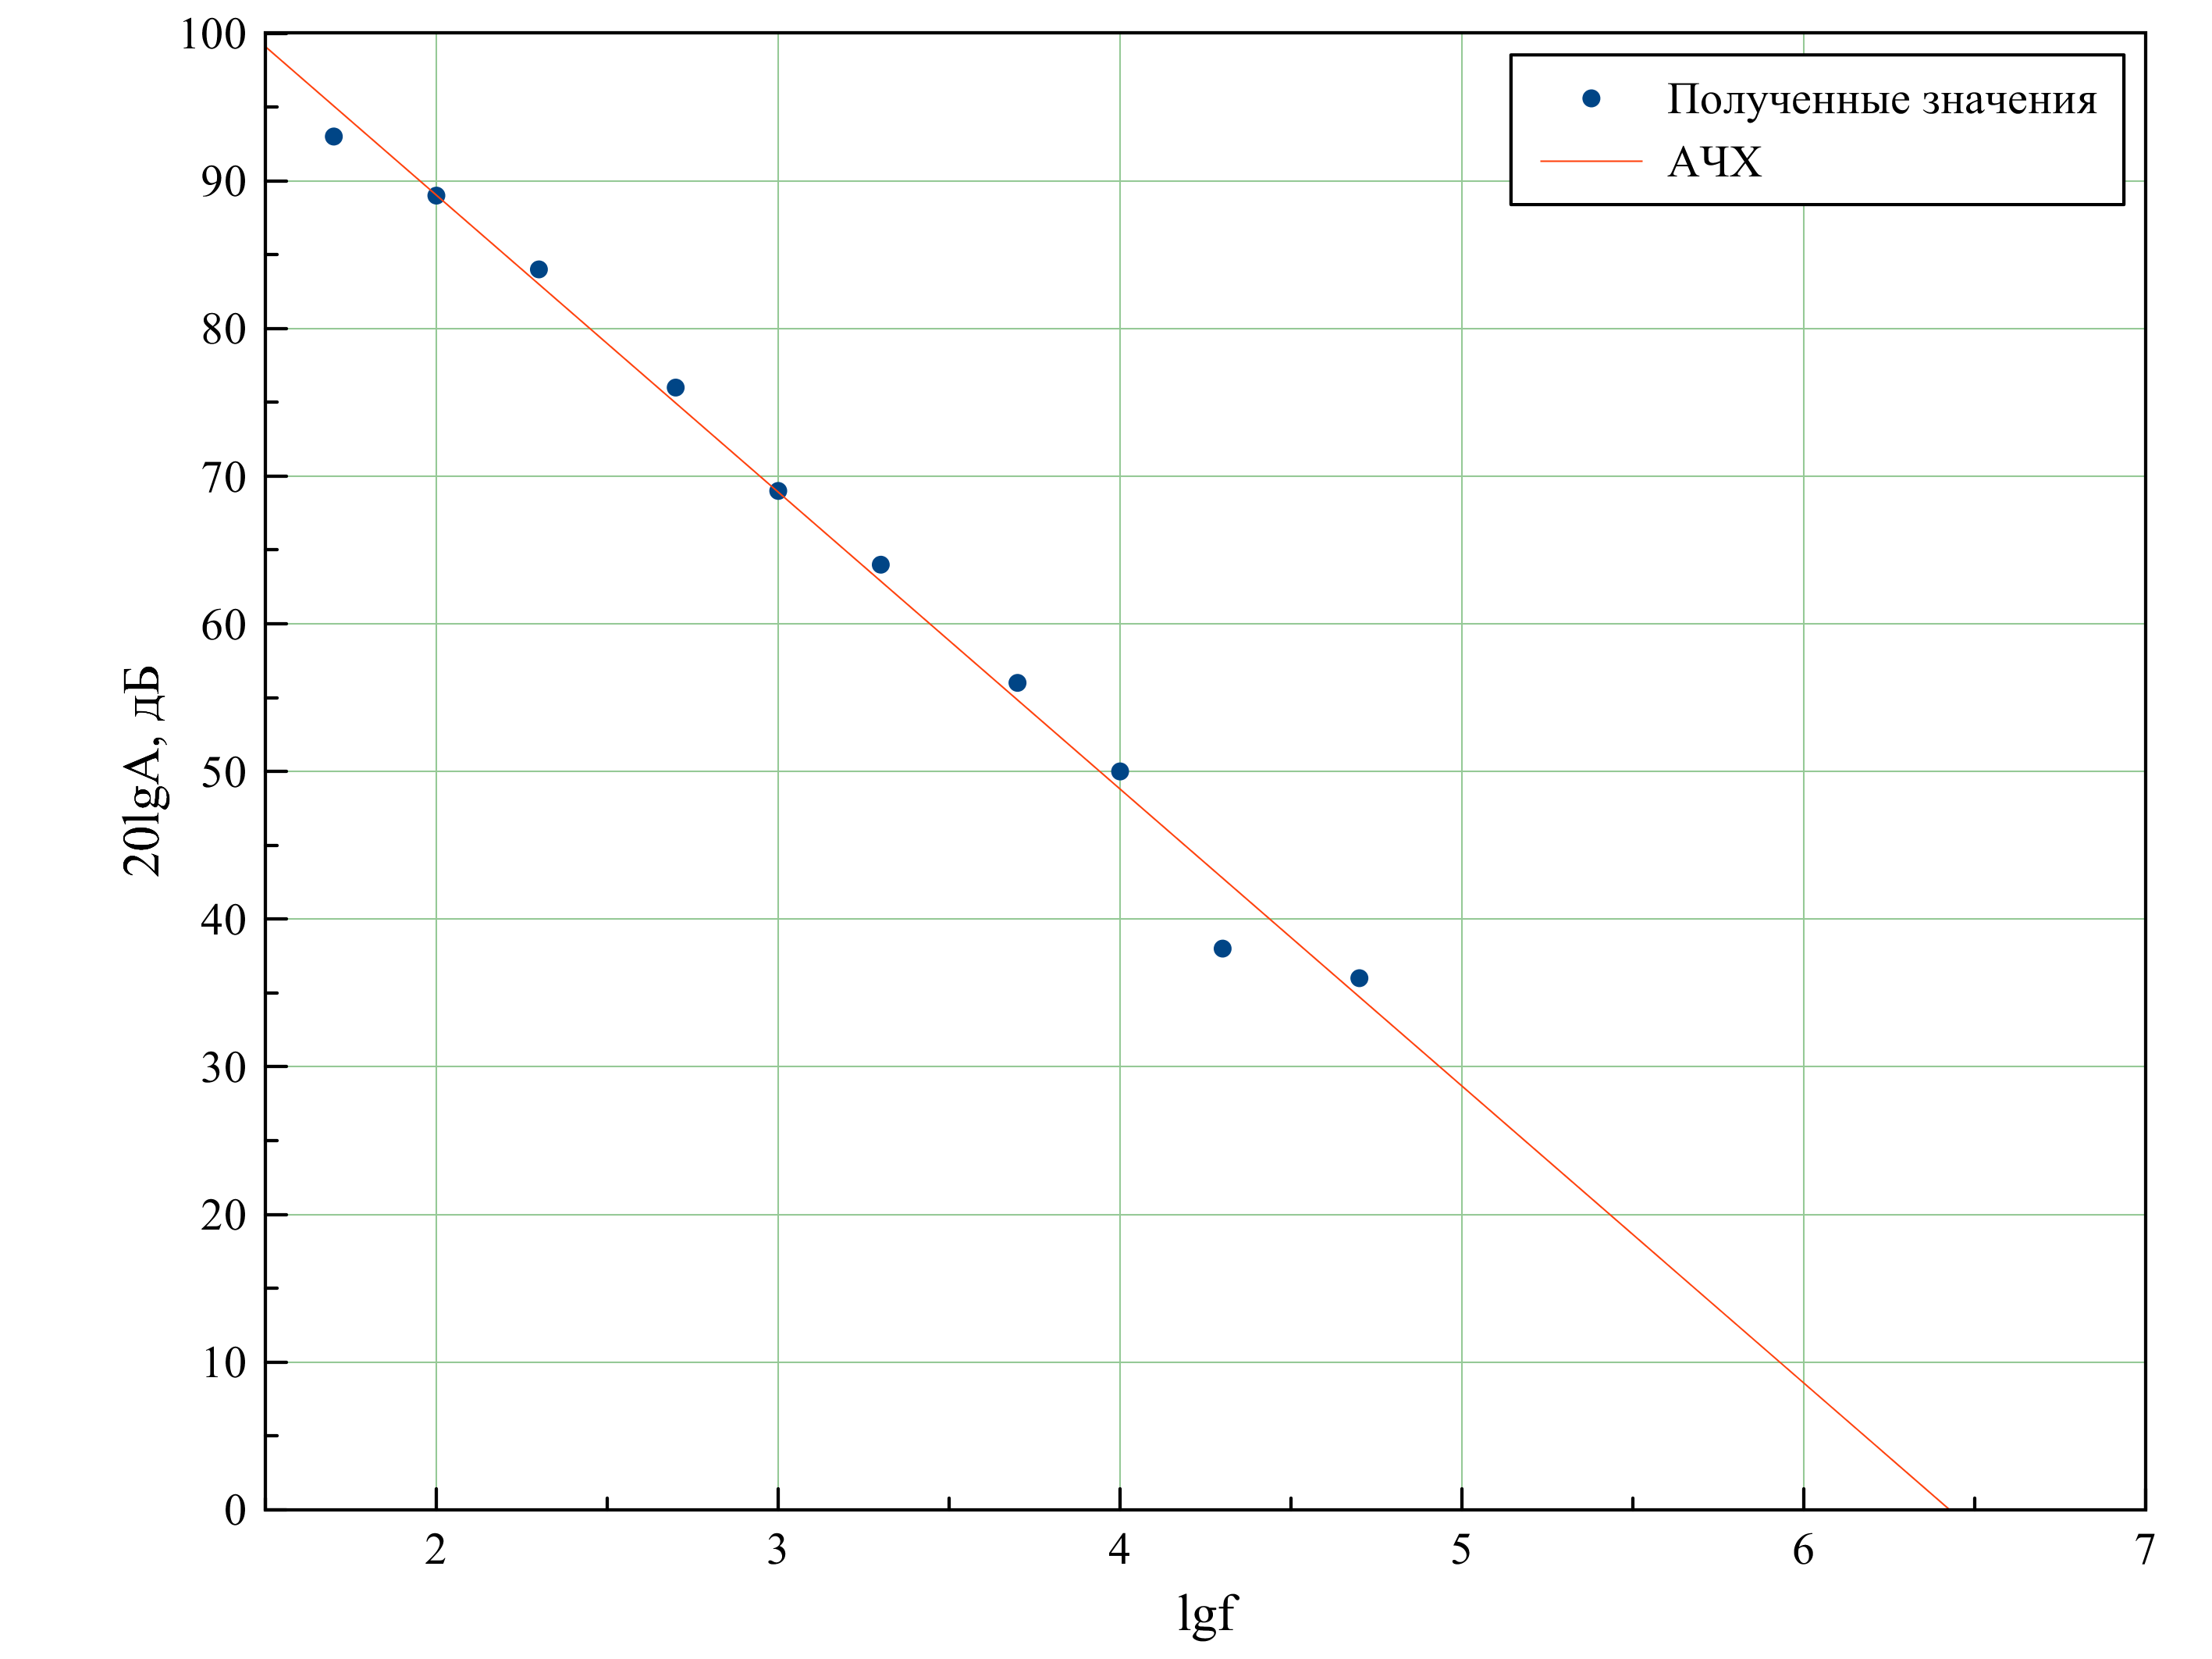
\includegraphics[width =  0.8\linewidth]{1}
	\caption{ АЧХ ОУ.}
	\label{ACHX}
\end{figure}

Из  рис. \ref{ACHX} получаем следующие величины:
$$f_T \simeq 3~ \text{МГц}, f_{p_0} \simeq 45~ \text{кГц} $$.
На частотах $f > f_{p_0}$ усиление падает обратно пропорционально частоте - с крутизной спада $-20$ дб/декада.

\section*{Задание №3. Неинвертирующий усилитель.}

\begin{figure}[H]
	\centering
	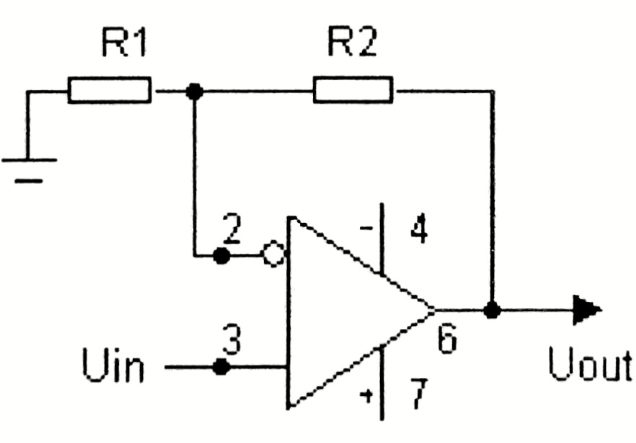
\includegraphics[width =  0.3\linewidth]{nus}
	\caption{Схема неинвертирующего усилителя.}
	\label{nus}
\end{figure}

Соберём схему, возьмём $R_1 = 2$ кОм, $R_2 = 200$ кОм, $R_2/R_1 = 100$.
\vspace{\baselineskip}

Измерим постоянное напряжение на выходе $U_{out(dc)} \simeq 68$ мВ. Определим входное напряжение сдвига ОУ: $U_{OS} = U_{out(dc)}/(1+R_2/R_1).$ Получим $U_{OS} \simeq 68/(1 + 100)\simeq 673$ мкВ.
\vspace{\baselineskip}

Снимем зависимость от частоты коэффициента усиления $K(f)$ при $U_{\text{вх}} = 10$ мВ. Полученные данные занесём в таблицу \ref{kust}.

\begin{table}[H]
	\centering
	\caption{Зависимость коэффициента усиления $K(f)$.}
	\label{kust}
	\resizebox{\textwidth}{!}{%
	\begin{tabular}{c|c|c|c|c|c|c|c|c|c|c|c|c|c|c|c}
		\toprule
		$f,$ Гц             & 50   & 100  & 200  & 500  & 1k   & 2k   & 5k   & 10k  & 20k & 50k  & 100k & 150k & 300k & 500k & 1M   \\ 
		$U_{\text{вых}},$ В & 1.04 & 1.04 & 1.04 & 1.04 & 1.04 & 1.03 & 1.02 & 0.97 & 0.9 & 0.55 & 0.31 & 0.21 & 0.11 & 0.07 & 0.03 \\ 
		K                   & 104  & 104  & 104  & 104  & 104  & 103  & 102  & 97   & 90  & 55   & 31   & 21   & 11   & 7    & 3    \\ \bottomrule
	\end{tabular}%
}
\end{table}

\begin{figure}[H]
	\centering
	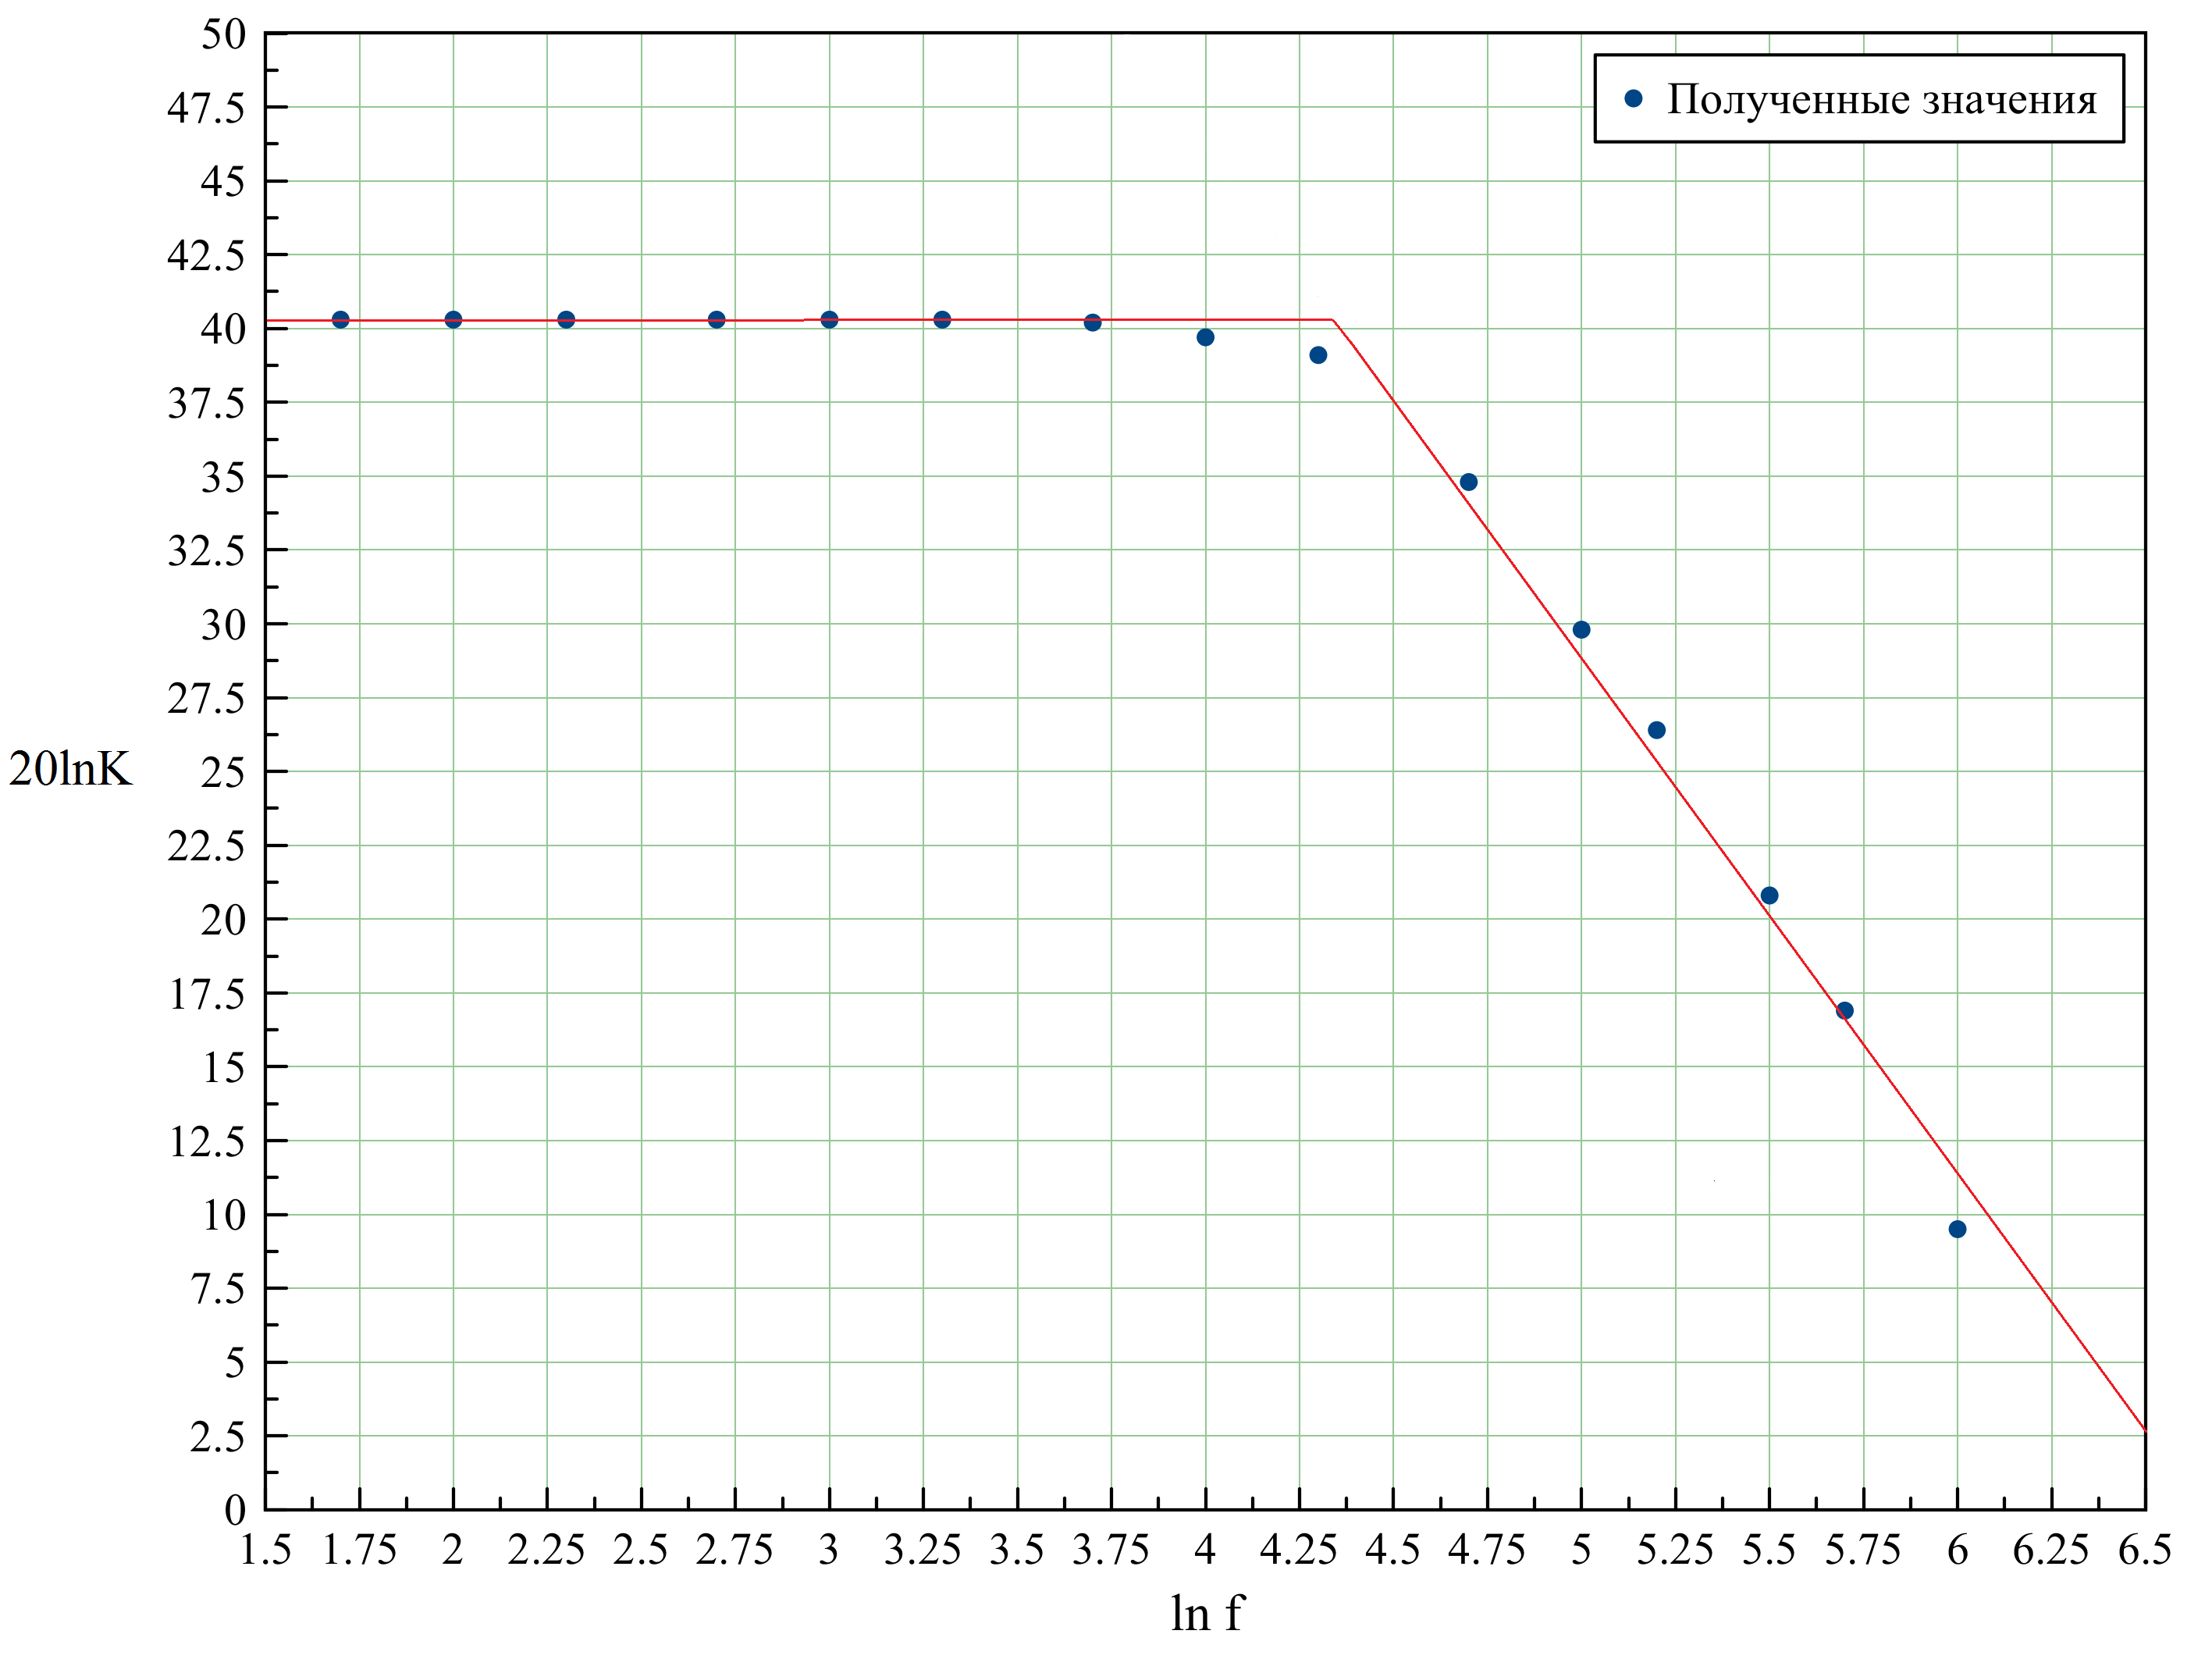
\includegraphics[width =  0.5\linewidth]{3}
	\caption{Зависимость коэффициента усиления $K(f)$.}
	\label{kf}
\end{figure}

Из рис. \ref{kf} определим граничную частоту $F_p$ по уровню $0.7$ относительно коэффициента усиления на низких частотах. Получим $F_p \simeq 31.6$ кГц.
\vspace{\baselineskip}

Проверим, что коэффициент усиления на низких частотах ($f < F_p$) и граничная частота усилителя удовлетворяет соотношениям: $K_0 = 1/\beta = 1+R_2/R_1;~ F_p = \beta f_T,~ \beta \hm{=} R_1/(R_1+R_2)$ - коэффициент отрицательной обратной связи.

$$\beta = 2/(2+200) \simeq 0.01 $$  
$$K_0 = 1/0.01 = 100 \simeq 101 = 1 + 200/2$$
$$31.6 \cdot 10^3 \simeq 0.01\cdot 3 \cdot 10^6$$

Все соотношения выполняются.
\vspace{\baselineskip}

Определим максимальную амплитуду неискажённого выходного напряжения на низкой частоте $f = 1.5$ кГц. Получим $U_{\text{вых}} \simeq 3.2$ В.
\vspace{\baselineskip}

Включим ОУ по схеме повторителя ($R_1 = \infty,~R_2 = 0$). Измерим коэффициент передачи и граничную частоту усилителя. Определим на частоте $f = 0.8$ МГц максимальную амплитуду неискажённого сигнала и характер искажений, возникающих при дальнейшем увеличении амплитуды входного сигнала. Получим $U_{m\_out} \simeq 3.0$ В. ("скошенная синусоида").
\begin{table}[H]
	\centering
	\caption{Зависимость коэффициента передачи повторителя.}
	\label{zk}
	\resizebox{\textwidth}{!}{%
	\begin{tabular}{c|c|c|c|c|c|c|c|c|c|c|c|c|c|c|c|c}
		\toprule
		$f,$ Гц             & 50   & 100  & 200  & 500  & 1k   & 2k   & 5k   & 10k  & 20k  & 1M   & 2M   & 2.5M & 2.6M & 3.4M & 5M   & 10M  \\ 
		$U_{\text{вых}},$ В & 1.00 & 1.00 & 1.00 & 1.00 & 1.00 & 1.00 & 1.00 & 1.00 & 0.98 & 1.00 & 1.05 & 1.00 & 1.00 & 0.99 & 0.60 & 0.31 \\ 
		K                   & 1.00 & 1.00 & 1.00 & 1.00 & 1.00 & 1.00 & 1.00 & 1.00 & 0.98 & 1.00 & 1.05 & 1.00 & 1.00 & 0.99 & 0.60 & 0.31 \\ \bottomrule
	\end{tabular}%
	}
\end{table}

\begin{figure}[H]
	\centering
	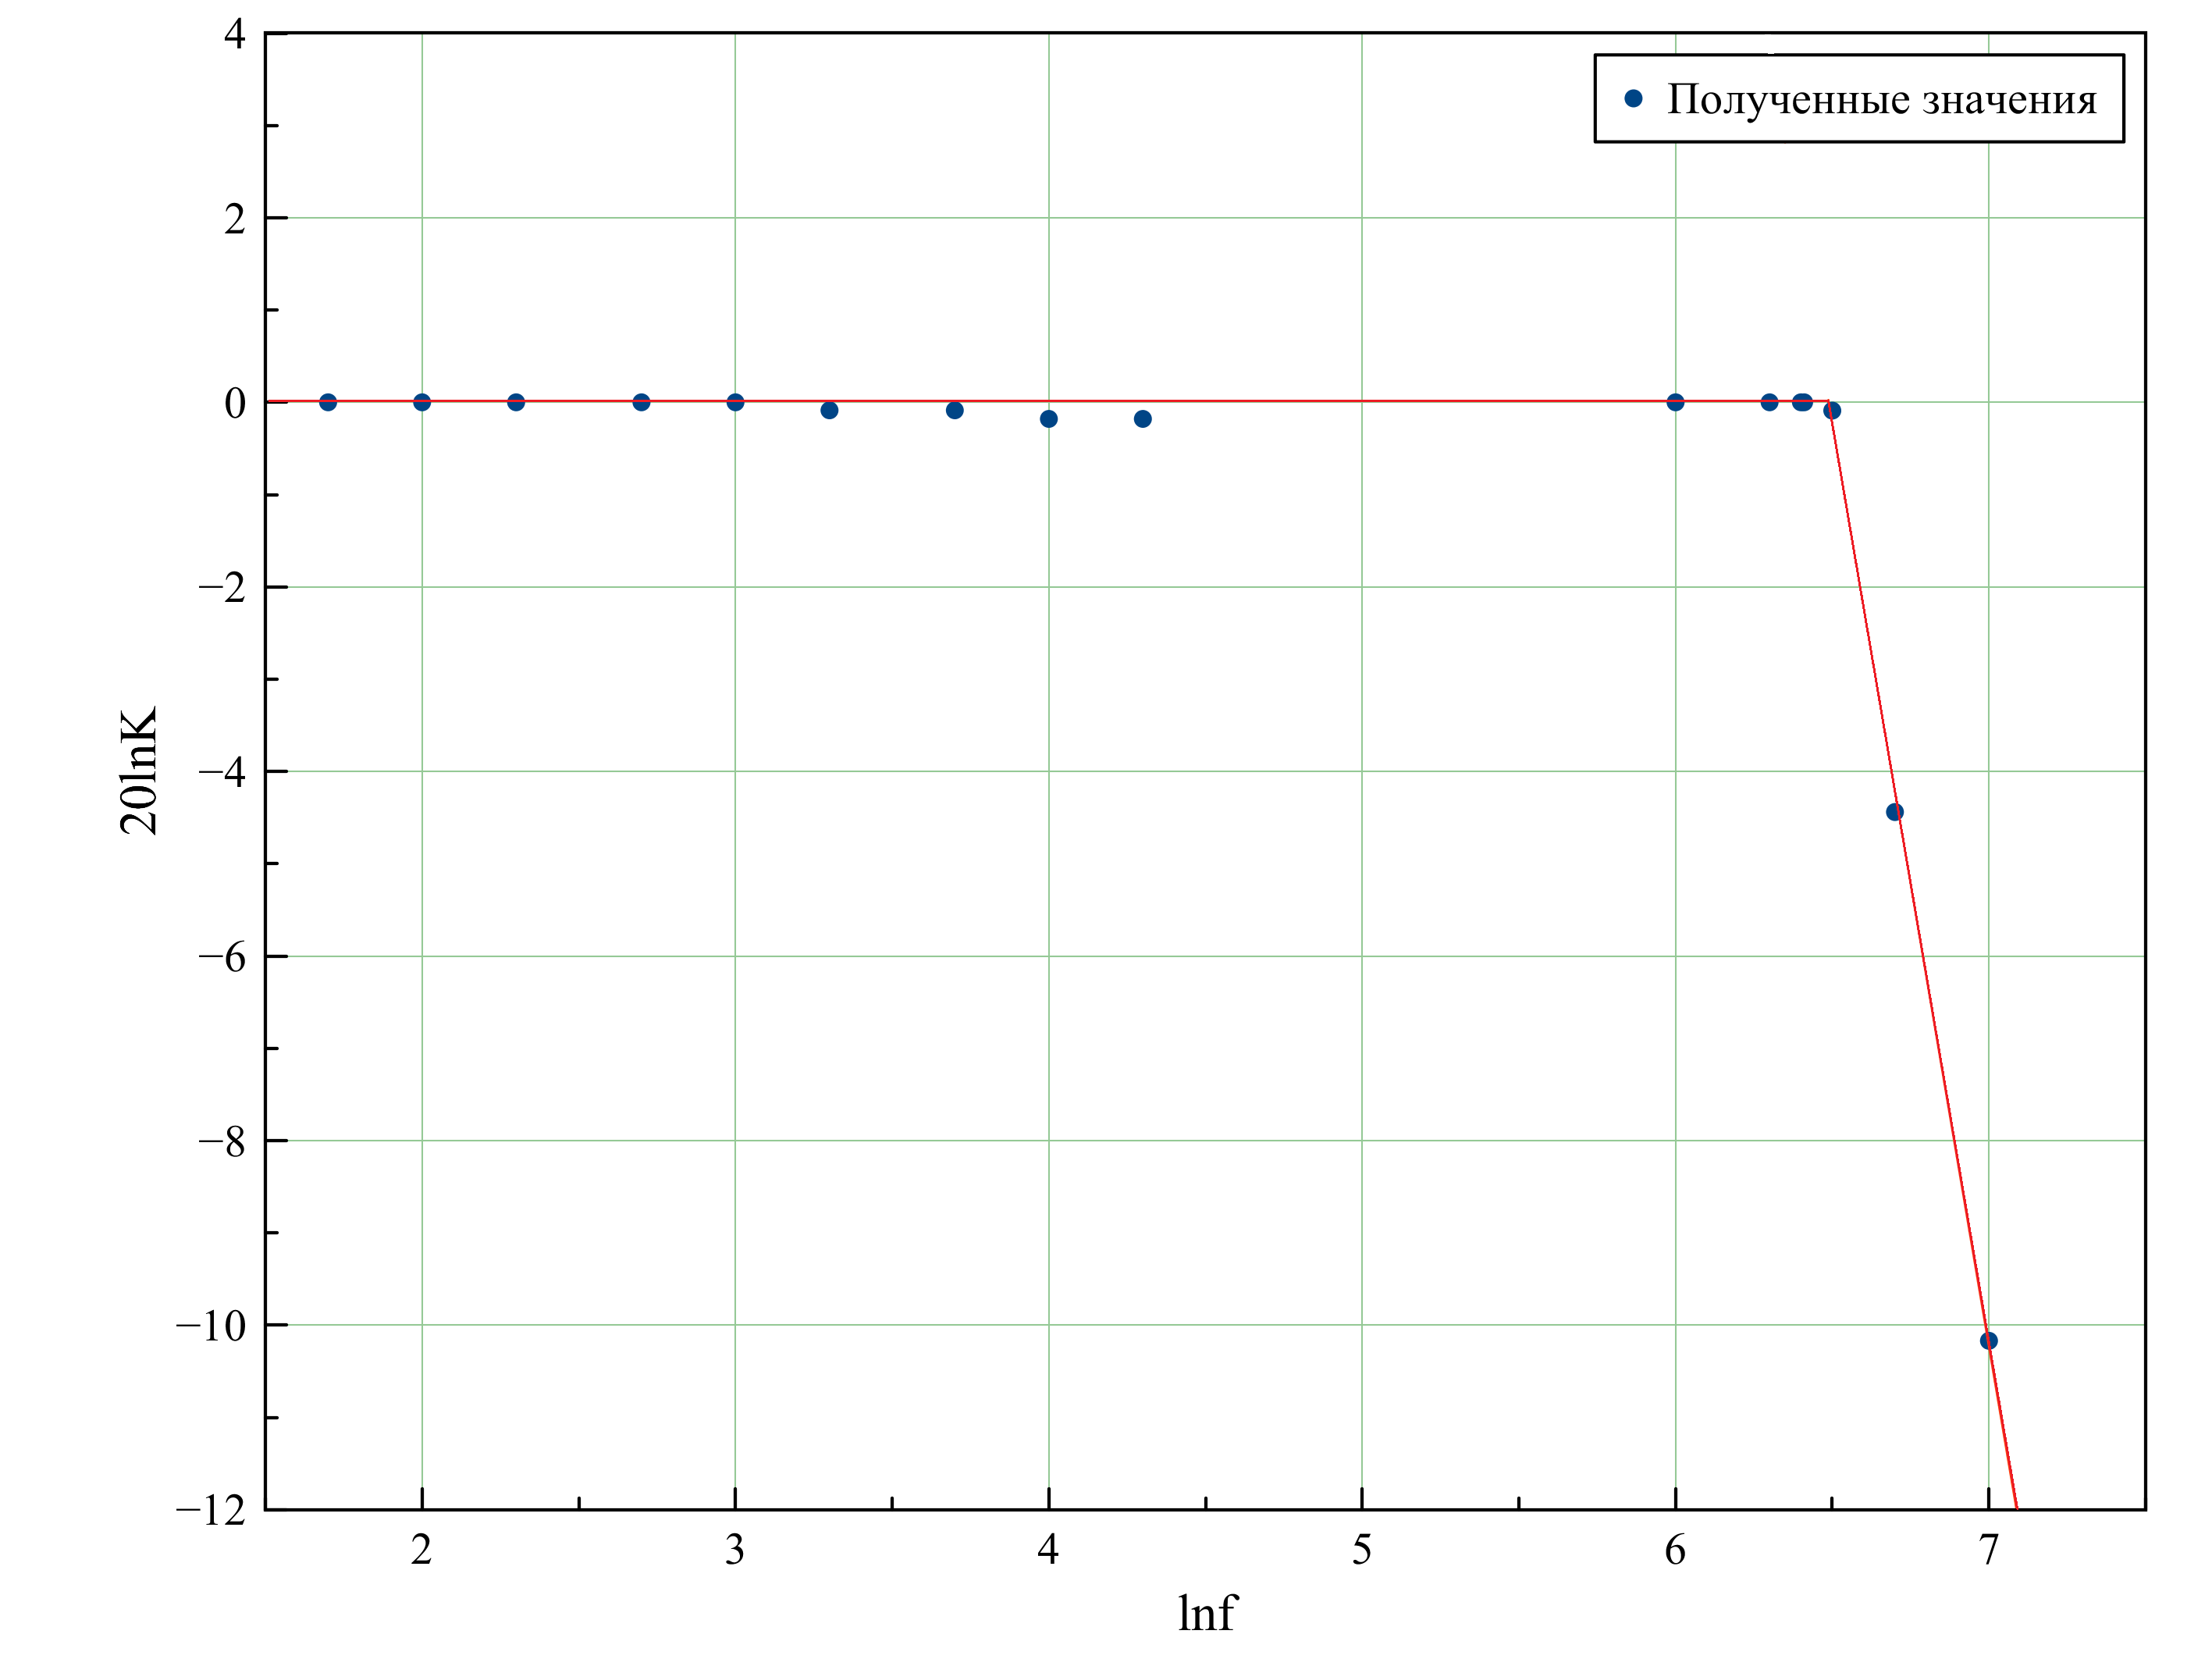
\includegraphics[width =  0.7\linewidth]{31}
	\caption{Зависимость коэффициента усиления $K(f)$ повторителя.}
	\label{kfp}
\end{figure}

Из рис. (\ref{kfp}) получаем, что граничная частота равна $f \simeq 3$ МГц.
\vspace{\baselineskip}

Сравним результат измерения максимальной амплитуды неискажённого сигнала с расчётом по формуле $U_{m\_out} = V_{max}/2\pi f$.
\vspace{\baselineskip}

$$ U_{m\_out} = \dfrac{ 13\cdot 10^6}{2\pi \cdot 0.8 \cdot 10^6} \simeq  2.6~\text{В} \approx 3.0 ~ \text{В}$$ 

\section*{Задание №4. Инвертирующий усилитель.}

\begin{figure}[H]
	\centering
	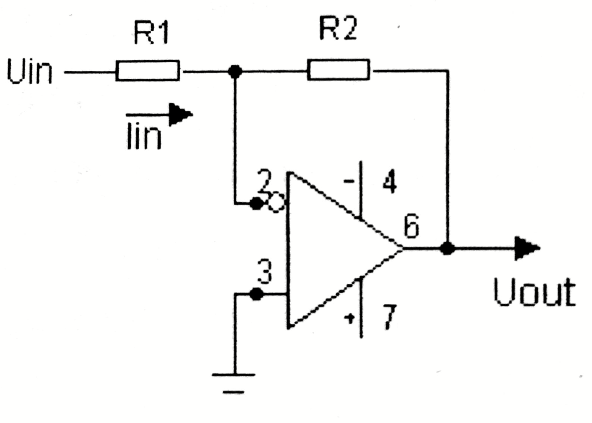
\includegraphics[width =  0.3\linewidth]{IMG_0662}
	\caption{Схема инвертирующего усилителя.}
	\label{schinv}
\end{figure}


Соберём схему, используя те же резисторы, что в задании №3; определим коэффициент усиления $K_0$ и граничную частоту $F_p$. Получим $K_0 = -\frac{97.2 \cdot 10^{-2}}{10^{-2}} = -97.2, ~ F_p \simeq 31.8\text{кГц}$ .

Также получим, что коэффициент усиления $K_0 = -\frac{R_2}{R_1} = - \frac{200 \cdot 10^3}{2\cdot 10^3} = -100$ и частота $F_p$ имеют те же значения, что и для неинвертирующего усилителя.
\newpage
\section*{Задание №10.1. Фильтр нижних частот.}

\begin{figure}[H]
	\centering
	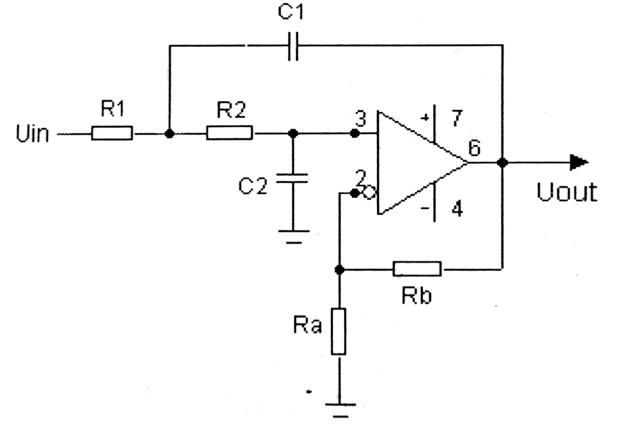
\includegraphics[width =  0.3\linewidth]{IMG_0663}
	\caption{Схема фильтра нижних частот.}
	\label{schinv}
\end{figure}

По заданным значениям частоты среза $f_c = 0.8$ кГц и коэффициента затухания $\alpha = 1.5$ рассчитаем и соберём схему: $C = (0.43 - 0.51)$ мкФ, $R = 510$ Ом, $R_b = 100$ Ом, $R_a\hm{=} 200 ~\text{Ом}$.

Снимем амплитудно-частотную характеристику фильтра.

\begin{table}[H]
	\centering
	\caption{АЧХ фильтра нижних частот ($\alpha = 1.5$).}

	\begin{tabular}{c|cccccccccccc}\toprule
		$f$, Гц & 50   & 100  & 200  & 500  & 700  & 800  & 1k   & 1.1k & 1.5k & 2k   & 5k   & 10k  \\
		$K$     & 1.51 & 1.51 & 1.47 & 1.17 & 0.90 & 0.75 & 0.53 & 0.47 & 0.27 & 0.15 & 0.03 & 0.01 \\ \bottomrule
	\end{tabular}
\end{table}

\begin{table}[H]
	\centering

	\begin{tabular}{c|ccccccccccc}\toprule
		$f$, Гц & 20k & 25k & 50k  & 100k & 200k & 500k & 1M   & 2M   & 4M   & 10M  & 20M  \\
		$K$     & 0.01   & 0.01   & 0.01 & 0.02 & 0.04 & 0.08 & 0.13 & 0.17 & 0.19 & 0.19 & 0.18 \\ \bottomrule
	\end{tabular}

\end{table}

\begin{figure}[H]
	\centering
	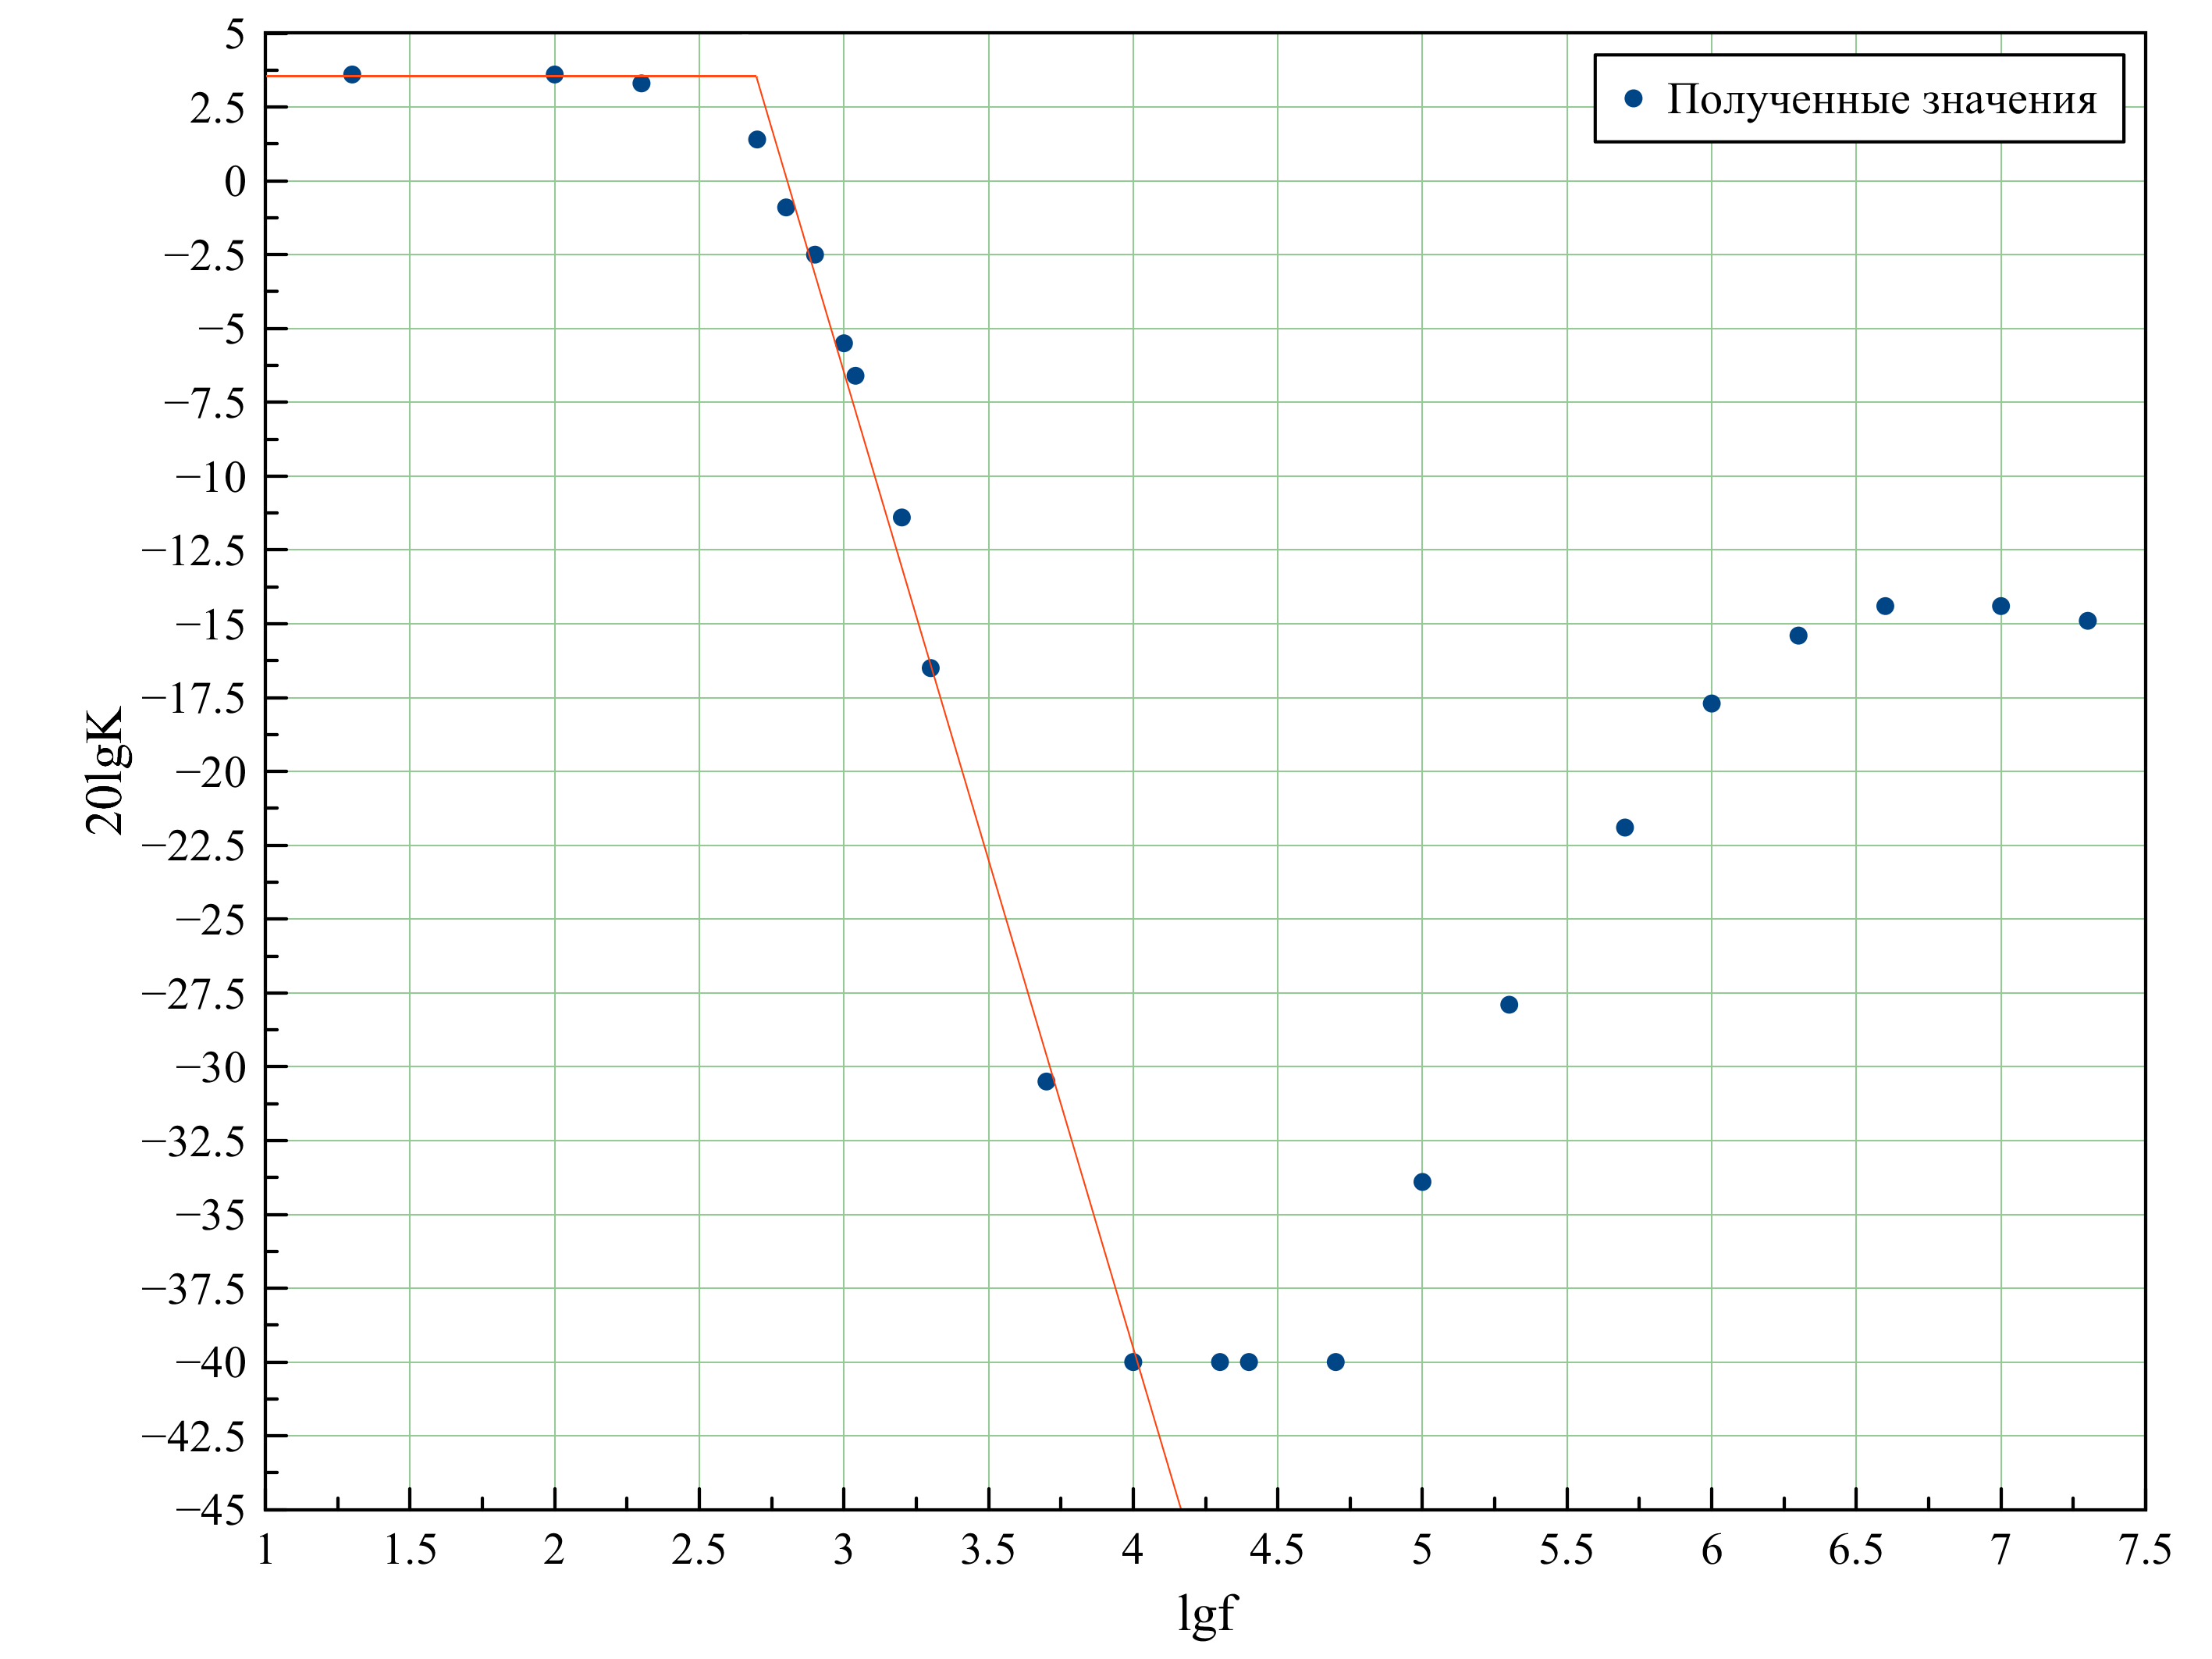
\includegraphics[width = 0.7\linewidth]{1011}
	\caption{АЧХ фильтра нижних частот ($\alpha = 1.5$).}
	\label{achxn4}
	
\end{figure}

Из рис.\ref{achxn4} получаем, что $f_c \simeq 600$ Гц, а крутизна спада на частотах $f>f_c$ составляет примерно $33.8$ дБ/дек.
\\

Изменим коэффициент затухания фильтра: $\alpha = 1 \rightarrow R_b = R_a = 100$ Ом. Повторим измерения.
\begin{table}[H]
	\centering
	\caption{АЧХ фильтра нижних частот ($\alpha = 1$).}
	
	\begin{tabular}{c|cccccccccccc}\toprule
		$f$, Гц & 50   & 100  & 200  & 500  & 700  & 800  & 1k   & 1.1k & 1.5k & 2k   & 5k   & 10k  \\
		$K$     & 2.01 & 2.03 & 2.09 & 2.23 & 1.73 & 1.39 & 0.92 & 0.76 & 0.39 & 0.22 & 0.03 & 0.01 \\ \bottomrule
	\end{tabular}
\end{table}

\begin{table}[H]
	\centering
	
	\begin{tabular}{c|ccccccccccc}\toprule
		$f$, Гц & 20k & 25k & 50k  & 100k & 200k & 500k & 1M   & 2M   & 4M   & 10M  & 20M  \\
		$K$     & 0.01   & 0.01   & 0.01 & 0.02 & 0.05 & 0.09 & 0.13 & 0.14 & 0.15 & 0.16 & 0.14 \\ \bottomrule
	\end{tabular}
	
\end{table}
\begin{figure}[H]
	\centering
	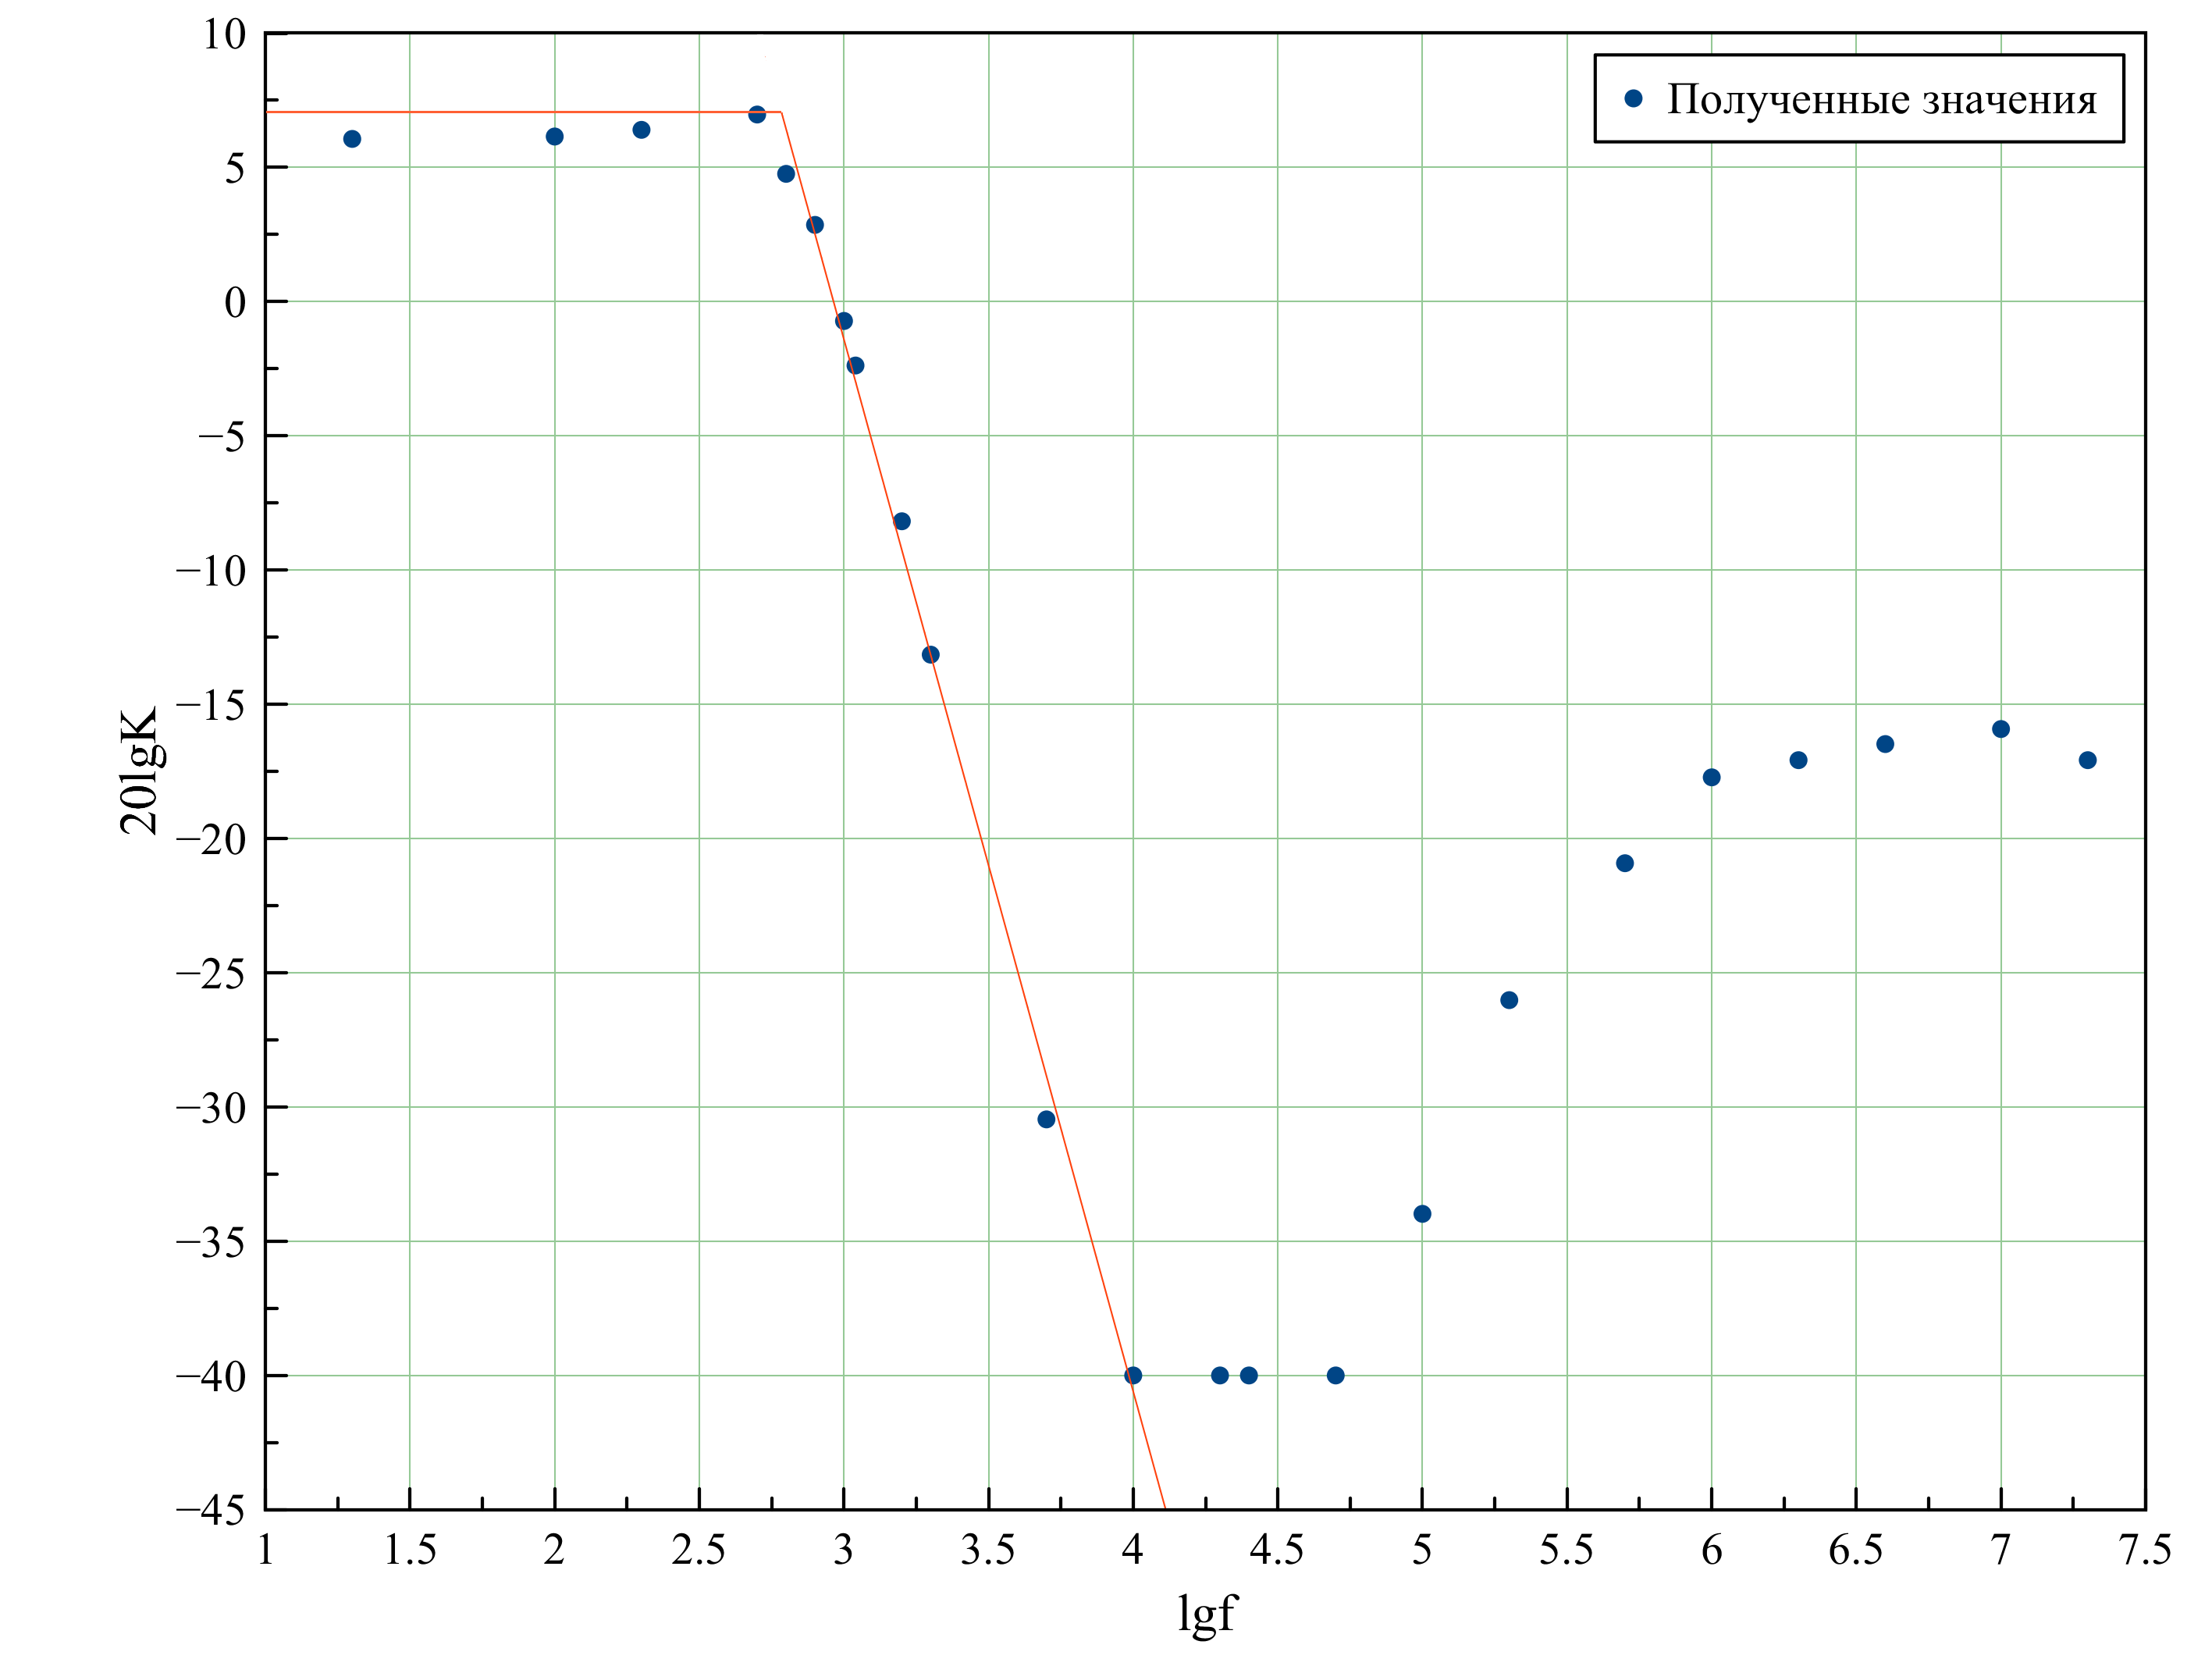
\includegraphics[width = 0.7\linewidth]{1012}
	\caption{АЧХ фильтра нижних частот ($\alpha = 1$).}
	\label{achxn41}
	
\end{figure}

Из рис.\ref{achxn41} получаем, что $f_c \simeq 630$ Гц, а крутизна спада на частотах $f>f_c$ составляет примерно $37.5$ дБ/дек.
\newpage
\section*{Задание №10.2. Фильтр верхних частот.}

\begin{figure}[H]
	\centering
	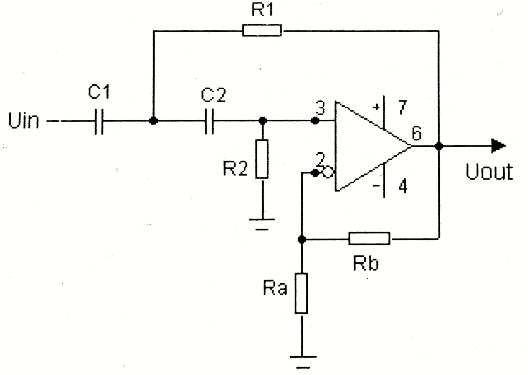
\includegraphics[width =  0.3\linewidth]{IMG_0664}
	\caption{Схема фильтра верхних частот.}
	
\end{figure}

По заданным значениям частоты среза $f_c = 0.8$ кГц и коэффициента затухания $\alpha = 1.5$ рассчитаем и соберём схему: $C = (0.43 - 0.51)$ мкФ, $R = 510$ Ом, $R_b = 100$ Ом, $R_a\hm{=} 200 ~\text{Ом}$.

Снимем амплитудно-частотную характеристику фильтра.

\begin{table}[H]
	\centering
	\caption{АЧХ фильтра верхних частот ($\alpha = 1.5$).}	
	
	\resizebox{\textwidth}{!}{
	\begin{tabular}{c|ccccccccccccccc}
		\toprule
		$f$, Гц & 50   & 100  & 200  & 500  & 1k   & 2k   & 5k   & 10k  & 20k  & 50k  & 100k & 200k & 500k & 1M   & 2M   \\
		$K$     & 0.01 & 0.03 & 0.13 & 0.69 & 1.23 & 1.38 & 1.42 & 1.42 & 1.41 & 1.41 & 1,41 & 1.39 & 1.27 & 1.05 & 0.62 \\ \bottomrule
	\end{tabular}
}
\end{table}

\begin{figure}[H]
	\centering
	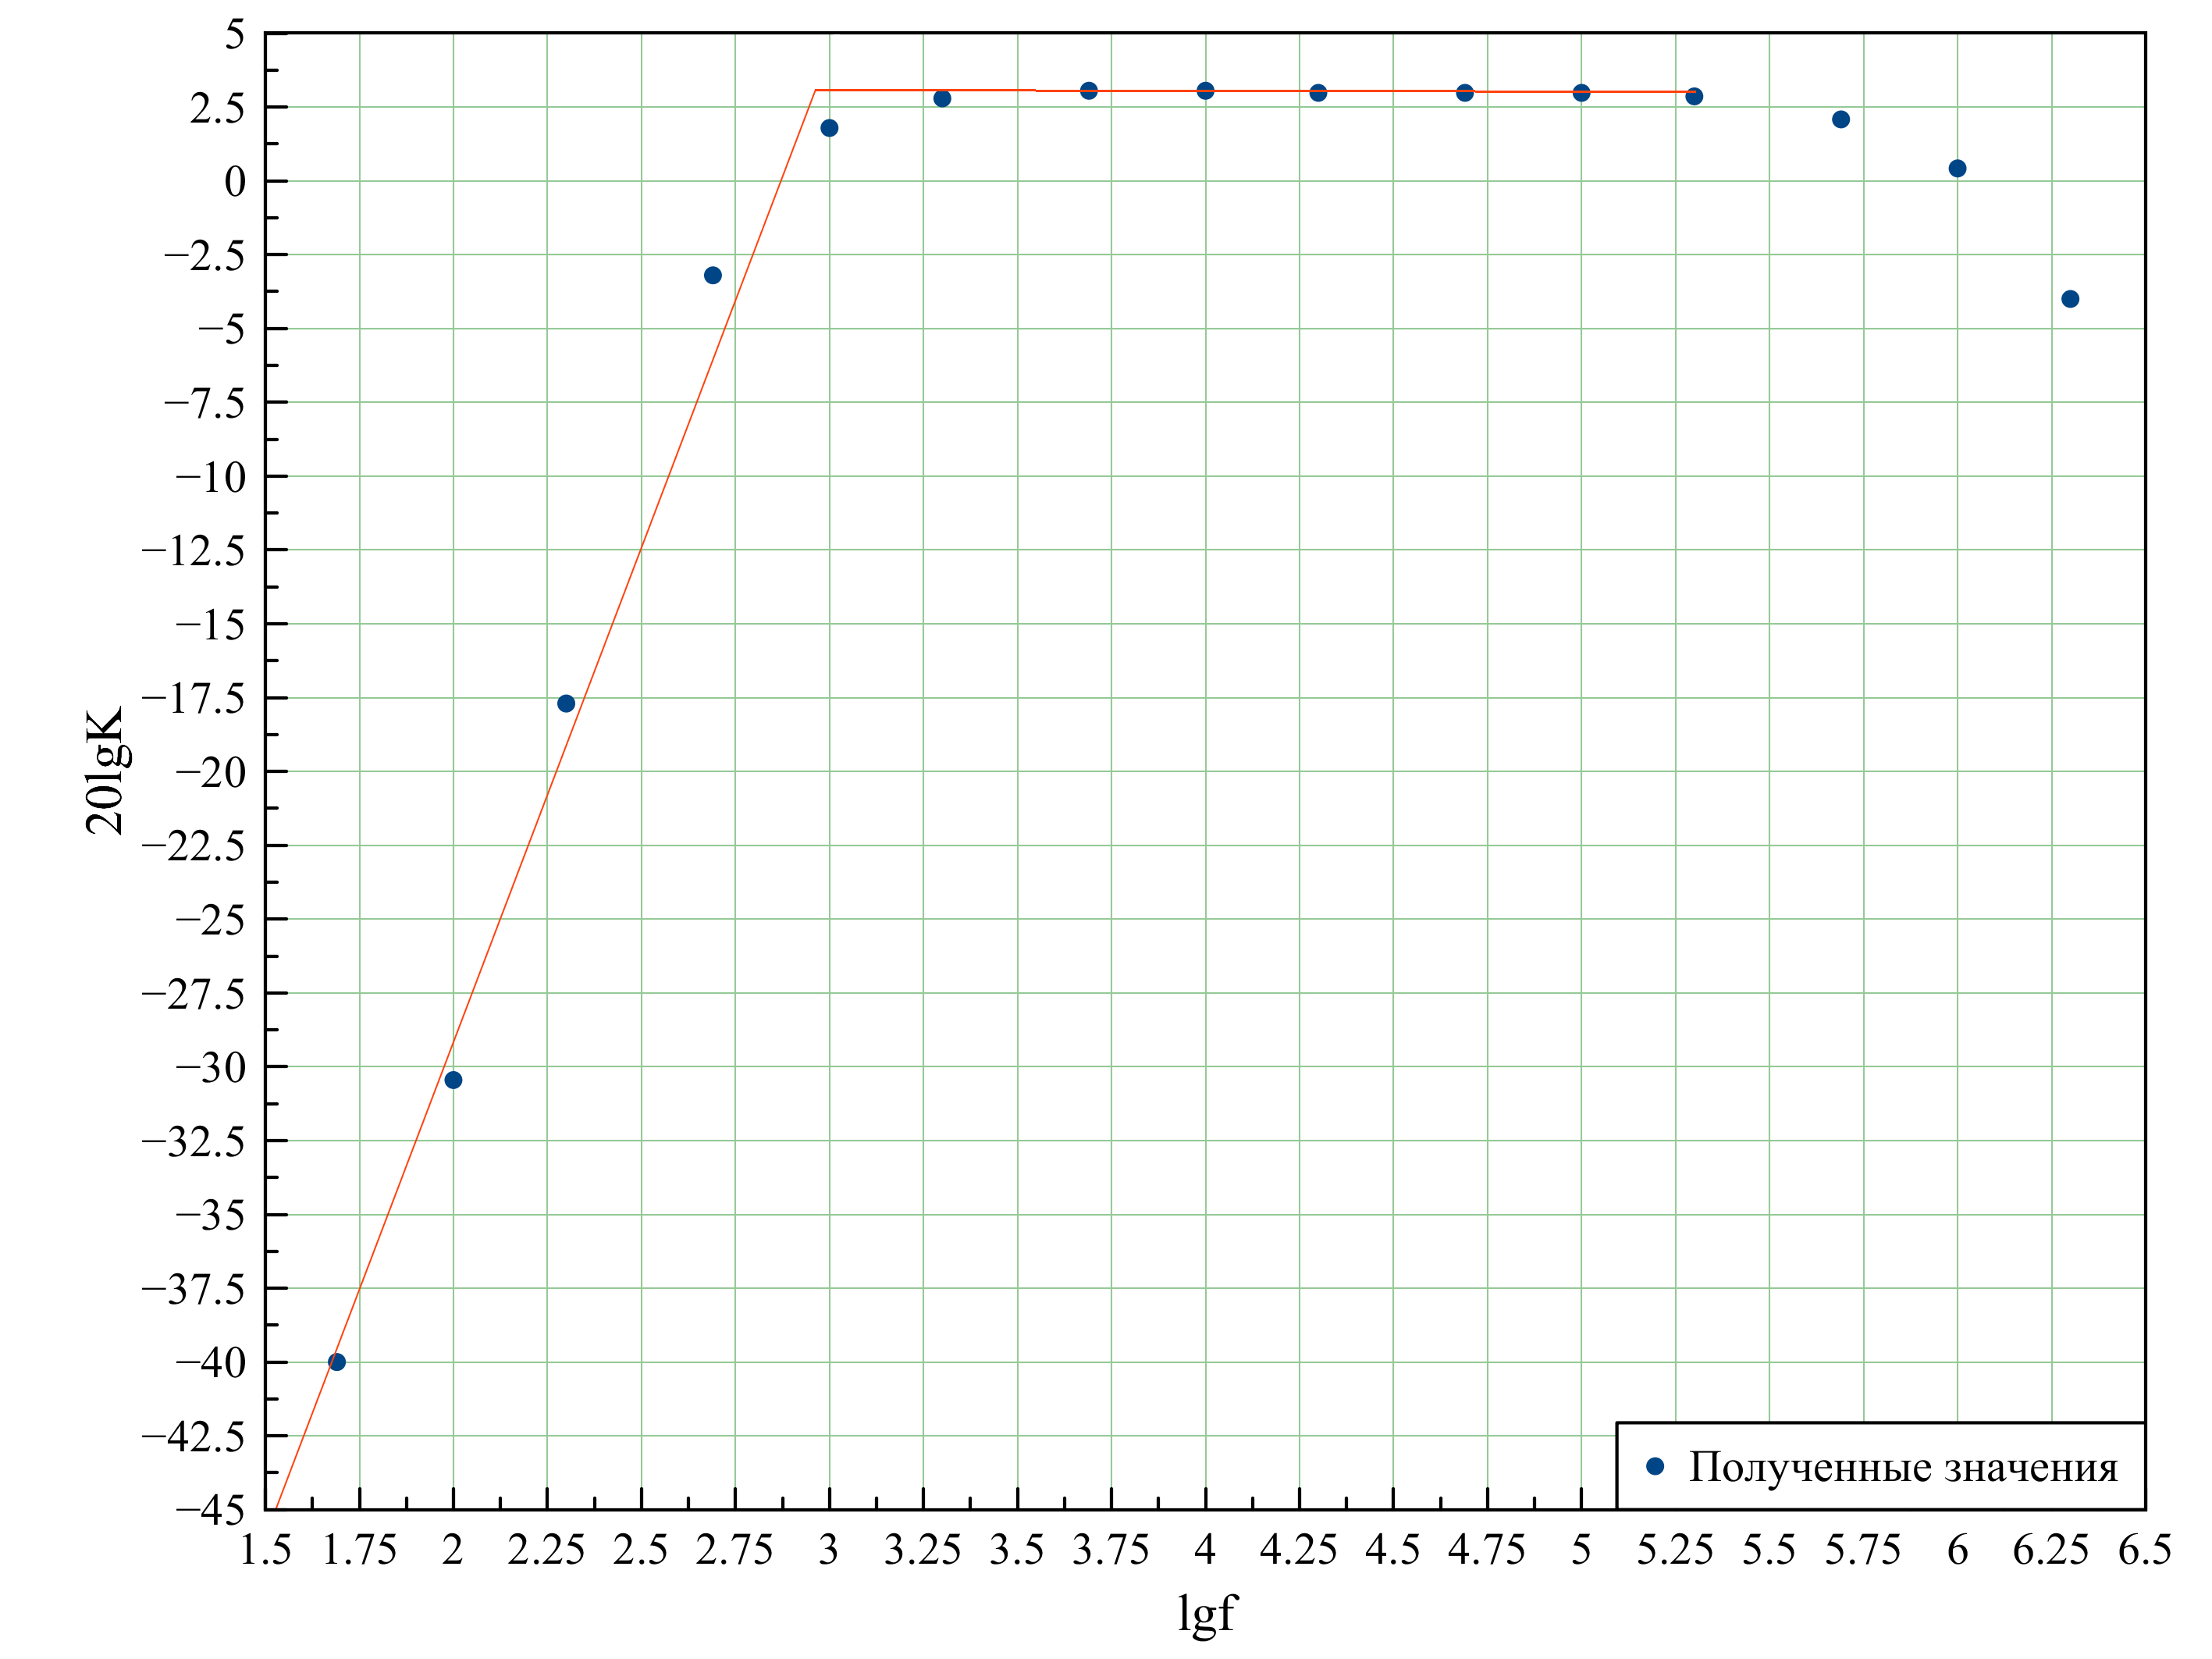
\includegraphics[width = 0.7\linewidth]{1021}
	\caption{АЧХ фильтра верхних частот ($\alpha = 1.5$).}
	\label{achxv4}
	
\end{figure}

Из рис.\ref{achxv4} получаем, что $f_c \simeq 800$ Гц, а крутизна нарастания на частотах $f<f_c$ составляет примерно $33.5$ дБ/дек. \\


Изменим коэффициент затухания фильтра: $\alpha = 1 \rightarrow R_b = R_a = 100$ Ом. Повторим измерения.

\begin{table}[H]
	\centering
	\caption{АЧХ фильтра верхних частот ($\alpha = 1$).}
		\resizebox{\textwidth}{!}{
	\begin{tabular}{c|ccccccccccccccc}
		\toprule
		$f$, Гц & 50   & 100  & 200  & 500  & 1k   & 2k   & 5k   & 10k  & 20k  & 50k  & 100k & 200k & 500k & 1M   & 2M   \\
		$K$     & 0.01 & 0.05 & 0.19 & 1.26 & 1.23 & 2.14 & 1.99 & 1.98 & 1.97 & 1.94 & 1.93 & 1.85 & 1.48 & 1.10 & 0.44 \\ \bottomrule
	\end{tabular}
}
\end{table}

\begin{figure}[H]
	\centering
	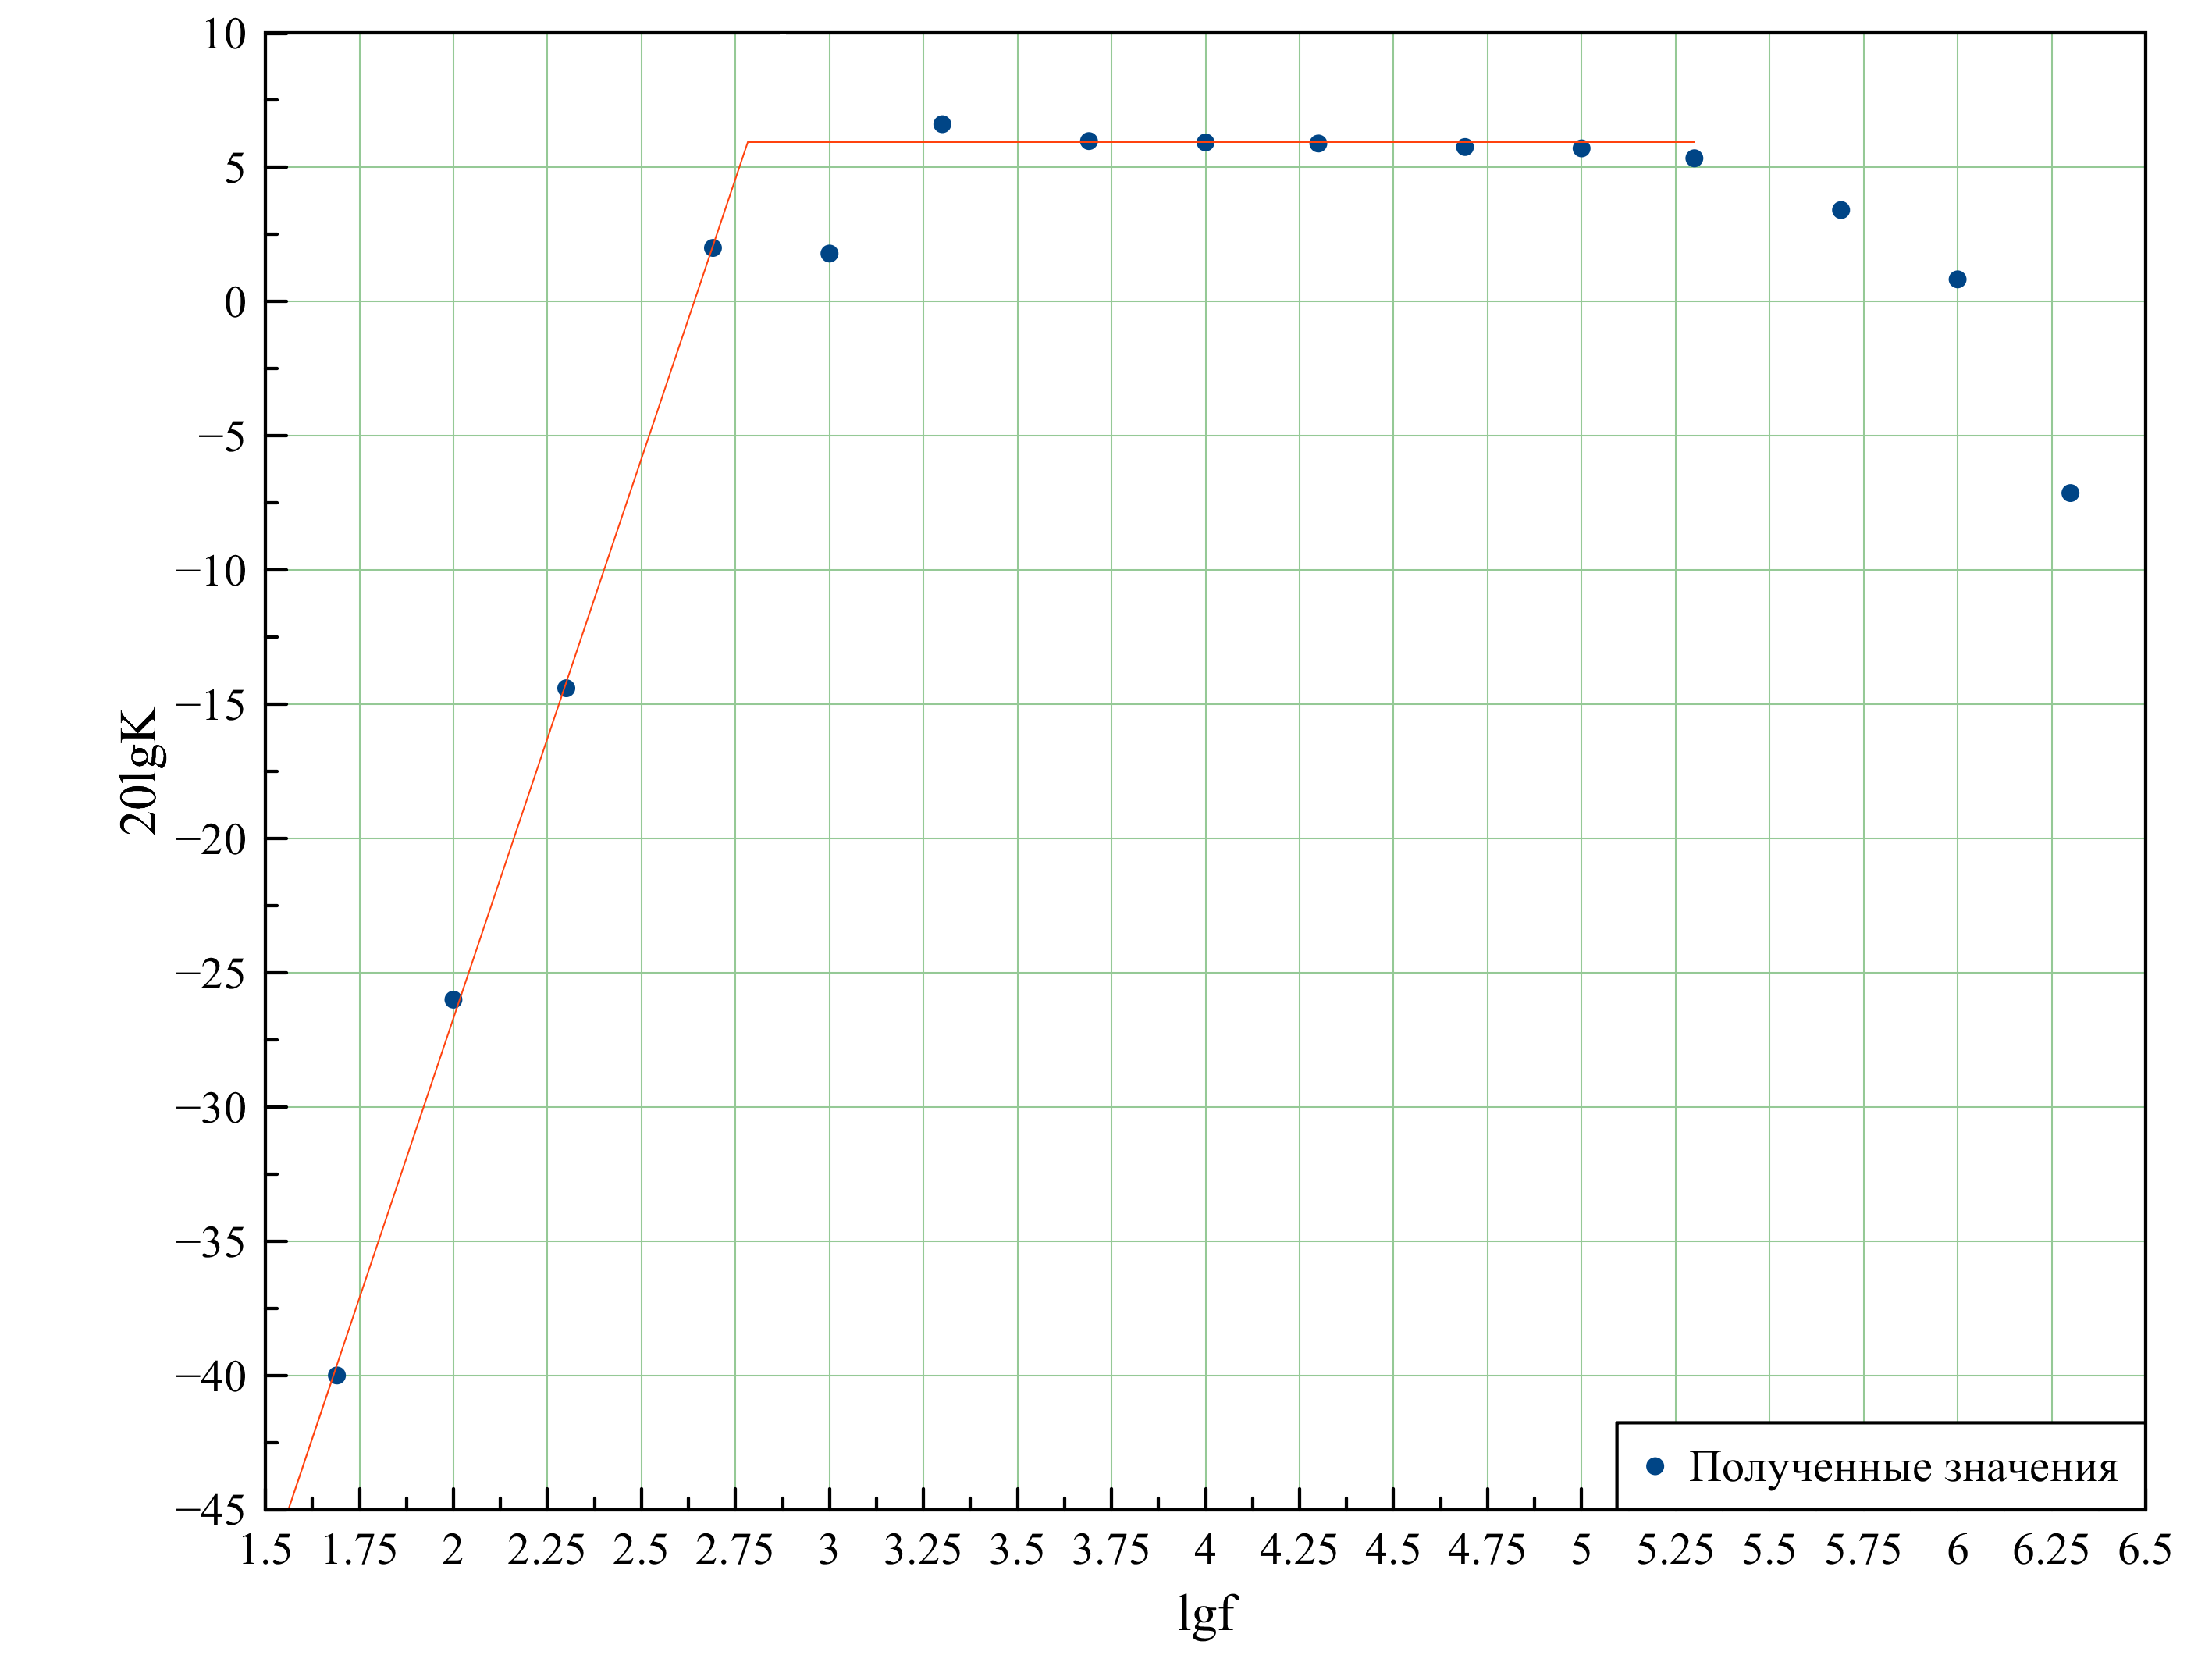
\includegraphics[width = 0.7\linewidth]{1022}
	\caption{АЧХ фильтра верхних частот ($\alpha = 1$).}
	\label{achxv41}
	
\end{figure}

Из рис.\ref{achxv41} получаем, что $f_c \simeq 630$ Гц, а крутизна нарастания на частотах $f<f_c$ составляет примерно $32.5$ дБ/дек. 

\newpage

\section*{Задание №10.3. Полосовой фильтр.}
\begin{figure}[H]
	\centering
	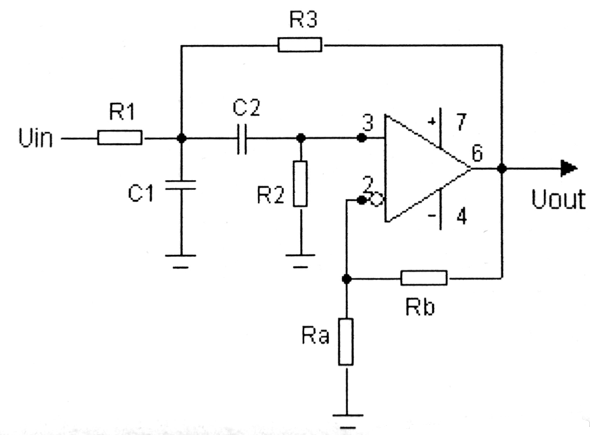
\includegraphics[width =  0.3\linewidth]{IMG_0665}
	\caption{Схема полосового фильтра.}
	
\end{figure}

По заданным значениям центральной частоты $f_0 = 800~\text{Гц}$ и полосы пропускания $\Delta f_{0.7} = 1.2 ~\text{кГц}$ рассчитаем и соберём схему: $C = (0.43 - 0.51) ~\text{мкФ}, ~ R_1=R_3=R\hm{=}510~\text{Ом},~R_2 = 2R\simeq 1~\text{кОм},~ R_b = 100~\text{Ом},~ R_a = 200~\text{Ом}.$ \\

Снимем амплитудно-частотную характеристику фильтра. Построим график АЧХ. Определим полосу пропускания, а также крутизну нарастания и спада.

\begin{table}[H]
	\centering
	\caption{АЧХ полосового фильтра.}
	\begin{tabular}{c|cccccccccccc}
		\toprule
		$f$, Гц & 5    & 10   & 50   & 100  & 200  & 400  & 500  & 600  & 700  & 800 & 900  & 1k    \\
		$K$     & 0.01 & 0.03 & 0.14 & 0.28 & 0.58 & 1.29 & 1.64 & 1.84 & 1.85 & 1.7 & 1.56 & 1.38  \\ \bottomrule
	\end{tabular}
\end{table}

\begin{table}[H]
	\centering
	\begin{tabular}{c|ccccccccccc}
		\toprule
		$f$, Гц & 1.1k & 1.5k & 2k   & 2.5k & 3k   & 4k   & 5k   & 6k   & 7k   & 8k   & 12k  \\
		$K$     & 1.26 & 0.88 & 0.65 & 0.51 & 0.42 & 0.31 & 0.25 & 0.22 & 0.18 & 0.16 & 0.11 \\ \bottomrule
	\end{tabular}
\end{table}

\begin{figure}[H]
	\centering
	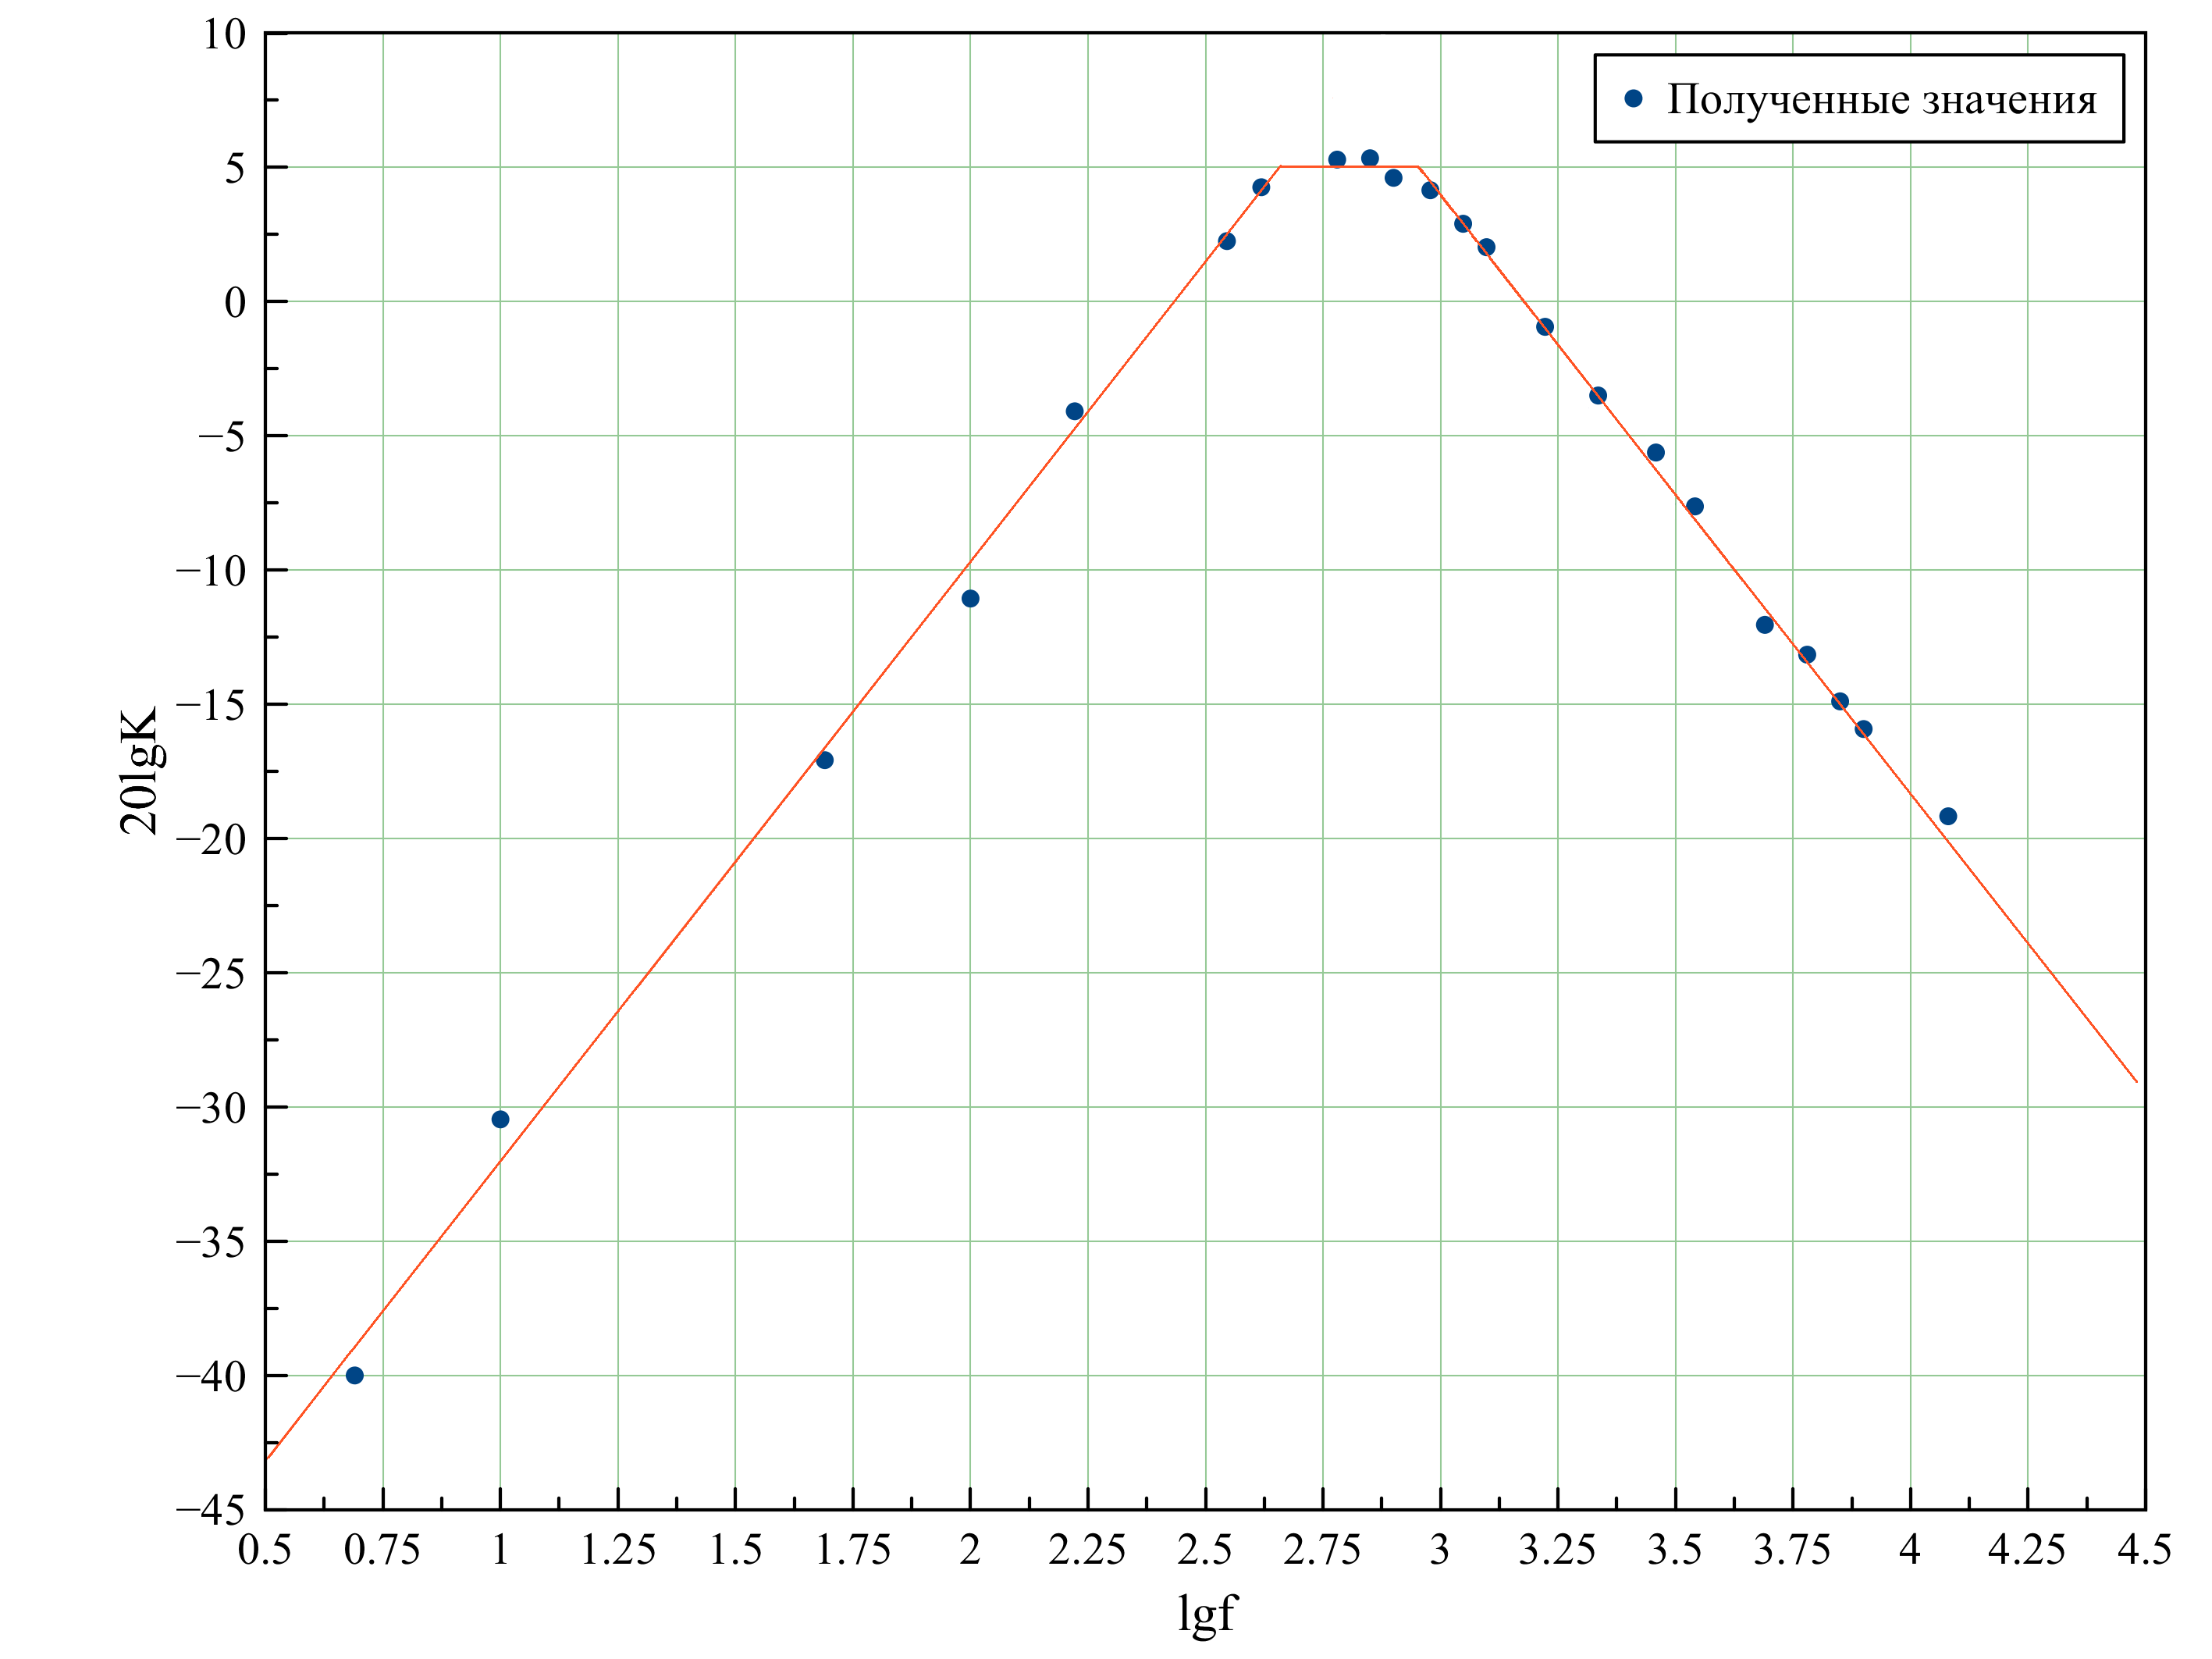
\includegraphics[width = 0.6\linewidth]{103}
	\caption{АЧХ полосового фильтра.}
	\label{achxp41}
	
\end{figure}
Из рис. \ref{achxp41} следует, что $\Delta f_{0.7} \simeq 600~\text{Гц}$. Крутизна нарастания равна $22.5$ дБ/дек, а крутизна спада - $16$ дБ/дек.
\newpage

\section*{Задание №11. Схемы с двойным T-образным мостом.}

\subsection*{11.1. Избирательный усилитель.}

\begin{figure}[H]
	\centering
	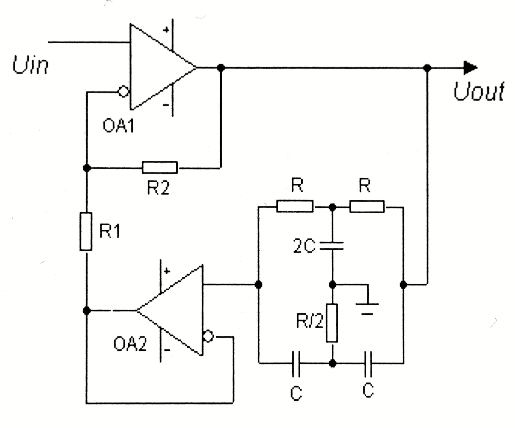
\includegraphics[width =  0.4\linewidth]{IMG_0667}
	\caption{Схема избирательного усилителя с двойным Т-образным мостом.}
	
\end{figure}

Исследование проводится с помощью программы \textit{Micro-Cap}.

\begin{center}
Центральная частота $f_0 \hm{\approx} 994$ Гц.
\end{center}

\begin{table}[H]
	\centering
	\begin{tabular}{c|cccc}
		\toprule
		$K = R_2/R_1$ & 50 & 100 & 150   & 200\\
		$Q = (K+1)/4$ & 12.75 & 25.25 & 37.75 & 50.25\\	$\Delta f_{0.7} = f_0/Q$&78& 39 & 26& 20 \\
		$\Delta f_{0.7_{\text{эксп}}}$&77&40&20&16\\ \bottomrule
	\end{tabular}
\end{table}

\subsection*{11.2. Режекторный фильтр.}
\begin{figure}[H]
	\centering
	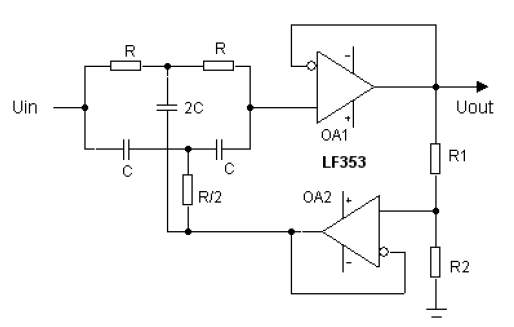
\includegraphics[width =  0.5\linewidth]{112}
	\caption{Схема режекторного фильтра с двойным T-образным мостом.}
	
\end{figure}

Исследование проводится с помощью программы \textit{Micro-Cap}.

\begin{center}
	Центральная частота $f_0 \hm{\approx} 1$ кГц.
\end{center}

\begin{table}[H]
	\centering
	\begin{tabular}{c|ccc}
		\toprule
		$K = R_2/(R_1+R_2)$ & 0.96 & 0.97 & 0.98   \\
		$\Delta f_{0.7} =4(1-K)\cdot f_0 $&160& 120 & 80\\
		$\Delta f_{0.7_{\text{эксп}}}$ &141&72&50\\ \bottomrule
	\end{tabular}
\end{table}





\end{document}
